\documentclass[a4paper]{article} 
\addtolength{\hoffset}{-2.25cm}
\addtolength{\textwidth}{4.5cm}
\addtolength{\voffset}{-3.25cm}
\addtolength{\textheight}{5cm}
\setlength{\parskip}{0pt}
\setlength{\parindent}{0in}

\usepackage{blindtext} % Package to generate dummy text
\usepackage{charter} % Use the Charter font
\usepackage[utf8]{inputenc} % Use UTF-8 encoding
\usepackage{microtype} % Slightly tweak font spacing for aesthetics
\usepackage[english]{babel} % Language hyphenation and typographical rules
\usepackage{amsthm, amsmath, amssymb} % Mathematical typesetting
\usepackage{float} % Improved interface for floating objects
\usepackage[final, colorlinks = true, 
linkcolor = black, 
citecolor = black]{hyperref} % For hyperlinks in the PDF
\usepackage{graphicx, multicol} % Enhanced support for graphics
\usepackage{xcolor} % Driver-independent color extensions
\usepackage{marvosym, wasysym} % More symbols
\usepackage{rotating} % Rotation tools
\usepackage{subcaption}
\usepackage{censor} % Facilities for controlling restricted text
\newcommand{\note}[1]{\marginpar{\scriptsize \textcolor{red}{#1}}} % Enables comments in red on margin
\usepackage{bm}
\usepackage{blkarray}
\usepackage{enumitem}
\usepackage{pgfplots}
\definecolor{colkeyword}{rgb}{0,0.4,0}
\definecolor{colname}{rgb}{0.4,0.4,0}
\definecolor{coltype}{rgb}{0.4,0,0.4}
\definecolor{coloperators}{rgb}{0,0,1.0}
\definecolor{colscopes}{rgb}{0.4,0,0}

\setcounter{tocdepth}{2}
% Title Page
\title{Summary Natural Language Processing 1}
\author{Phillip Lippe}


\begin{document}
\maketitle
\tableofcontents
\newpage

\section{Morphology and finite state techniques}
\begin{itemize}
	\item Morphology concerns the \textbf{structure of words}
	\item \textit{Morpheme}: minimal information carrying unit in a word. A word consists of morphemes
	\item \textit{Affix}: Morphemes that only occur in conjunction with other morphemes
	\item \textit{Stem}: a word is made up of a stem and zero or more affixes. Stems are therefore stand-alone morphemes
	\item There are different forms of affixes that describe when (prefix, suffix, infix, ...)
	\item An affix is productive if it applies in general and therefore also probably for new words
	\item \textbf{Inflectional morphology}
	\begin{itemize}
		\item Fills predefined slots in paradigm, as plural, tense,... (create different grammatical forms, but word stays the same)
		\item Fully productive, except irregular forms
		\item Inflectional affixes are not combined in English
	\end{itemize}
	\item \textbf{Derivational morphology}
	\begin{itemize}
		\item Forming a new word through affix (also change of meaning possible)
		\item May change POS tag
		\item Examples include \textit{anti-}, \textit{re-}, \textit{-ism}, \textit{-ist} (``reset'' vs. ``set'')
		\item Generally semi-productive (applies for only subset of words in language)
		\item Include \textit{zero-derivation}: word that is both verb and noun, e.g. ``text'' vs. ``(to) text (someone)''
	\end{itemize}
	\item Ambiguities in terms of morphemes (single stems or affixes are ambiguous like ``dog'') or structure (combination of affixes/stem like ``shorts'' vs ``short-s'')
	\item \textbf{Bracketing}
	\begin{itemize}
		\item Starting from the stem, find the combination of nearby affixes that still lead to a possible form
		\item Example \textit{un-ion-ise-ed}. Putting \textit{un-} and \textit{ion} together not possible as this forms a non-valid word (union would be different stem). $\Rightarrow$ \textit{un-(ion-ise)-ed}
		\item Next, adding the \textit{-ed} ending is valid, and finally concatenating it with \textit{un-}: \textit{(un-((ion-ise)-ed))}
	\end{itemize}
\end{itemize}
\subsection{Applications of morphological processing in NLP}
\begin{itemize}
	\item We can use morphology to create a full-form lexicon (lexicon with each form of every word in it). However, this tends to explode very fast (high redundancy) and is not scalable for new words
	\item \textbf{Stemming}: use rules to get the stem form of a word. This allows us to match words to a small set of base words
	\item \textbf{Lemmatization}: Only finding split of stems and affixes. Is the preprocessing step before parsing (understanding the word!)
	\item Morphological process can either by analysis or generation
	\item Possible aspects/steps of morphological processing
	\begin{enumerate}
		\item Surface/ground-word mapped to stem(s) and affixes. Either by declaring the affixes (\textit{ping-ed}) or by explicitly saying which rule was applied (\textit{ping} \textit{PAST\_VERB})
		\item After knowing the affixes, analyze internal structure by bracketing
		\item Finally, understand syntactic and semantic effects where parsing can filter results of previous stages
	\end{enumerate}
	\item Overall, we need a lexicon combining three aspects:
	\begin{itemize}
		\item affixes (with the associated information they carry)
		\item irregular forms
		\item stems (with syntactic categories)
	\end{itemize}
\end{itemize}
\subsection{Spelling rules}
\begin{itemize}
	\item English morphology is essentially concatenative
	\item English spelling rules can be described independently of the particular stems and affixes involved. It simply looks at the affix boundaries.
	\item Example spelling rule for e-insertion:
	$$\epsilon \to \text{e}/\left\{\begin{array}{c}
	\text{s}\\
	\text{x}\\
	\text{z}
	\end{array}\right\}\hat{\text{ }}\textunderscore s$$
	Here, the formula is interpreted as ``an empty string maps to e if an s,x or z is followed by an s of the next affix'' (where e is inserted in the underscore space)
	\item Finite state machines (or transducers also creating corresponding output while parsing) can be used to implement spelling rules
	\begin{figure}[ht]
		\centering
		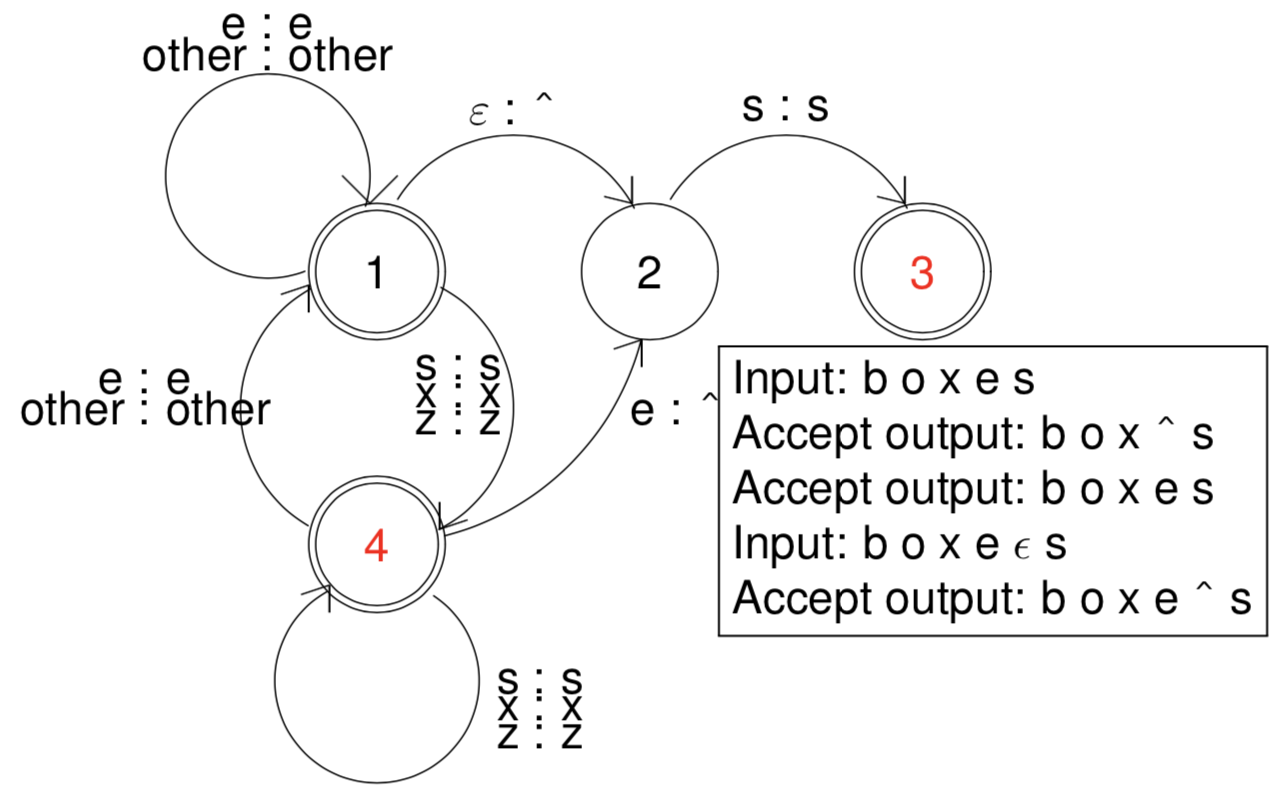
\includegraphics[width=0.4\textwidth]{figures/morphology_FST.png}
	\end{figure}
	\item Each transition corresponds to a pair of characters. 
	\item When the transducer is run in analysis mode, the system can detect an affix boundary (where we look up the stem and affix in the corresponding lexicon)
	\item In generation mode, we can just put in our parsed version and generate the correct spelling
	\item Morphology systems are usually implemented so that there is one FST per spelling rule and these operate in parallel
	\item However, FST are not applicable for internal structures as for example no bracketing model is possible
	\item A system which generates invalid output/accepts invalid derivations is said to \textbf{overgenerate}.
\end{itemize}
\section{Language models and part-of-speech tagging}
\subsection{Probabilistic language modeling}
\begin{itemize}
	\item The Naive Bayes approach considers words as independent. However, we can also model word sequences using statistical techniques (based on context/semantic and syntax)
	\item \textbf{Corpus}: text collected for some purpose (i.e. movie reviews)
	\begin{itemize}
		\item A corpus is \textit{balanced} if it represents different genres (types of text/domain)
		\item A \textit{tagged} corpus has annotations regarding the POS tags (mostly POS tags are learned unsupervised, but with this data we enable supervised training methods)
	\end{itemize}
	\item Use of language modeling
	\begin{itemize}
		\item In speech recognition, it is hard to distinguish between words that sound similar. Thus, language modeling is used to rank the hypothesis of the recognizing system to make an estimation what phrase is most likely being said
		\item Language modeling can also be used for word prediction, text entry, spelling correction, ...
	\end{itemize}
\end{itemize}
\subsubsection{N-gram models}
\begin{itemize}
	\item Modeling a sequence of $n$ words
	\item \textbf{Bigram} ($n=2$): 
	\begin{itemize}
		\item use only previous word $\Rightarrow$ $p(w_n|w_{n-1})$
		\item Probability of a sequence can be expressed by $p(w_1,...w_N)=\prod\limits_{n=1}^{N} p(w_n|w_{n-1})$
		\item Still, we assume that words with distance of more than 1 are independent
		\item Estimating the probabilities by the maximum likelihood solution: $$p(w_n|w_{n-1})=\frac{c(w_n, w_{n-1})}{\sum_{w_k} c(w_k, w_{n-1})}=\frac{c(w_n, w_{n-1})}{c(w_{n-1})}$$
		Thus, we normalize the counts over the next word $w_{n-1}$
	\end{itemize}
	\item \textbf{Trigram} ($n=3$):
	\begin{itemize}
		\item The probability of a word is based on the two previous words $\Rightarrow$ $p(w_n|w_{n-1},w_{n-2})$
		\item Again, the probability of the sequence is $p(w_1,...w_N)=\prod\limits_{n=1}^{N} p(w_n|w_{n-1},w_{n-2})$
	\end{itemize}
	\item Problems with sparse data
	\begin{itemize}
		\item \textbf{Smoothing}: for smoothing, we add a small extra probability for rare and unseen events to prevent probabilities of zero. E.g. for bigram:
		$$p(w_n|w_{n-1})=\frac{c(w_n, w_{n-1}) + \kappa}{c(w_{n-1}) + |V|\cdot \kappa }$$
		Simple to implement, but only suitable if having few unseen events (high $n$-gram have a lot)
		\item \textbf{Backoff}: If we have good evidence of a long phrase, we use a high $n$-gram model (for example trigram). Otherwise, if phrase was not seen yet, we go to the next smaller model (here bigram) and checker its probability. If also not known, go deeper until you reach unigram.
		\item \textbf{Interpolation}: combine the probability estimations of all models. For example we can use linear interpolation where we weight every model with a parameter:
		$$p(w_n|w_{n-1},w_{n-2}) = \lambda_1 p(w_n) + \lambda_2 p(w_n|w_{n-1}) + \lambda_3 p(w_n|w_{n-1}, w_{n-2})$$
		The parameters $\lambda_i$ need to sum up to 1 and are optimized on small held-out training subset. 
		\item \textbf{Unknown word tag}: using a unknown word tag which is also used in the training set. Replace all unknown words in the (test) text by this tag
	\end{itemize}
	\item Another limitation of $n$-gram models are long-term dependencies as these cannot be captured efficiently
	\item \textit{Evaluation} of $n$-gram models
	\begin{itemize}
		\item \textbf{Intrinsic evaluation}: evaluate directly on test set designed for the task with a metric
		\begin{itemize}
			\item A suitable metric is for example \textit{perplexity} which is the inverse probability of the test dataset normalized by number of words $N$:
			$$PP(W) = \left(p(w_1,...,w_N)\right)^{-1/N}$$
			\item For bigram, this would be $PP(W)=\left(\prod_{n=1}^{N}p(w_n|w_{n-1})\right)^{-1/N}$
			\item The goal is to minimize perplexity (lower perplexity indicates better model)
			\item However, perplexity strongly relies on the similarity of training and test dataset and is therefore not comparable across different datasets
		\end{itemize}
		\item \textbf{Extrinsic evaluation}: evaluation in the context of external task, i.e. speech recognition or word prediction
		\begin{itemize}
			\item Better, but very time consuming
			\item Hybrid approaches compare own models by perplexity, and apply the best model in extrinsic environment (external task)
		\end{itemize}
	\end{itemize}
\end{itemize}
\subsection{Part-of-speech tagging}
\begin{itemize}
	\item Tag every word by what king of speech it is (verb, noun, ... $\Rightarrow$ ambiguity)
	\item The tags are taken from a tagset which uses standardized codes for fine-grained POS
	\item \textit{Benefits} of POS tagging
	\begin{itemize}
		\item First step towards syntactic analysis (is very fast, but simpler than full syntax parsing)
		\item POS tags can be useful features for application
	\end{itemize}
	\item Problem of ambiguity: most high-frequency words have more than one POS tag. Language with rich morphology (significant affixes) tend to have less as the distinguish affixes better
\end{itemize}
\subsubsection{Tagging strategies}
\begin{itemize}
	\item Simplest strategy: assign to each words its most common tag (also called unigram tagging). Already gives a strong baseline
	\item \textbf{Hidden Marcov models}
	\begin{enumerate}
		\item Start with untagged text
		\item Assign to the words all their possible POS tags
		\item Find the most probable sequences of tags given sequences of words
		$$\hat{t}^{n} = \arg\max_{t^{n}} p(t^{n} | w^{n}) = \arg\max_{t^{n}} p(w^{n}|t^{n})\cdot p(t^{n}) $$
	\end{enumerate}
	\item If we apply for example bigram in this model, we get:
	\begin{equation*}
	\begin{split}
	p(t^{n}) & \approx \prod_{i=1}^{n} p(t_i | t_{i-1})\\
	p(w^{n}|t^{n}) & \approx \prod_{i=1}^{n} p(w_i | t_i)\\
	\hat{t}^{n} & = \arg\max_{t^{n}} \prod_{i=1}^{n}p(w_i | t_i)p(t_i | t_{i-1})
	\end{split}
	\end{equation*}
	\item Actual systems use trigrams. Smoothing and backoff are important (fewer unknown open class words)
	\item Evaluation by percentage of correct tags (but using most common tag already gives 90\% accuracy. With trigram about 97\%)
	\item Common errors
	\begin{itemize}
		\item Difference between country ``Turkey'' and bird ``turkey'' (it decides based on whether an \textit{a} is in front of turkey or not)
		\item Because of smoothing, we can get for the phrase ``have hope'' that both words are verbs although hope has no past tense which is antigrammatical!
	\end{itemize}
\end{itemize}
\section{Formal grammars and syntactic parsing}
\begin{itemize}
	\item Syntax: structure of sentence, parsing syntax to get (long-distance) dependencies of words
\end{itemize}

\subsection{Generative grammar}
\begin{itemize}
	\item Formally specified grammar that can generate all and only acceptable sentences of a natural language
	\item A phrase can be bracketed into its internal structure: \textit{((the (big dog)) slept)}
	\item Each subpart is a \textbf{constituent}: group of words/phrase behaving as a single unit 
	\item Labels can be assigned to the internal structures (for instance, \textit{the big dog} is a noun phrase)
\end{itemize}
\subsubsection{Phrases and substitutability}
\begin{itemize}
	\item Words with the same POS tag can be replaced
	\item Phrasal categories indicate which phrases can be substituted
	\item Example phrasal categories include noun phrase (NP), verb phrase (VP), propositional phrase (PP), ...
	\item Goal: capture substitutability at phrase level by phrasal categories
\end{itemize}
\subsection{Context-Free Grammars}
\begin{itemize}
	\item Defining a grammar on rules of production, and basic lexicon
	\item Basic elements of a context-free grammar (CFG):
	\begin{enumerate}
		\item Set of non-terminal symbols (e.g. S, VP)
		\item Set of terminal symbols (i.e., the words)
		\item Set of rules, where left-hand side is single non-terminal symbol, and right side combination of non-terminal and terminal. Examples:\\
		\texttt{S -> NP VP}\\
		\texttt{V -> fish}
		\item A start symbol (here \texttt{S}) which is a non-terminal
	\end{enumerate}
	\item Exclude empty productions, like \texttt{NP->$\epsilon$}
	\item For rules of non-terminal to single word, the non-terminal represents the POS tag of this word
	\item A context free grammar can be used for either generating sentences (start with \texttt{S}, and choose rules), or for analyzing/assigning a structure to a given sentence
	\item For analyzing, the bracketed notation or a parse tree is often used to represent the structure:
	
	\texttt{(S (NP} \textit{they}\texttt{) (VP (V }\textit{fish}\texttt{)))}  (for parse tree, \texttt{S} would be root node and \texttt{NP} and \texttt{VP} its children a.s.o.)
	\item However, the grammar is not always unique 
	\begin{itemize}
		\item \textbf{Lexical ambiguity}: a word is more than once in the lexicon having different POS tag
		\item \textbf{Structural ambiguity}: multiple possible analysis because of multiple rules for same non-terminals
	\end{itemize}
\end{itemize}
\subsection{Chart parsing with CFGs}
\begin{itemize}
	\item Increase efficiency by recording all possible rules we could apply on a sentence
	\item The \textbf{chart} is a record of all substructures that have ever been built during the parsing / stores partial results of parsing in a vector
	\item An \textbf{edge} is a data structure that represents a rule application ,which includes:
	\begin{itemize}
		\item An id for referring to it
		\item The outer left and right node in the sentence of the phrase on which the rule is applied
		\item The \textit{mother} symbol (non-terminal which is on the left side of the rule)
		\item The \textit{daughters} which are the symbols on the right side of the rule (words and/or non-terminals produced by previous edges and referred to by the id)
	\end{itemize}
	\item In conclusion, a full chart for the sentence \texttt{they can fish} look like that:
%	$$\begin{array}{ccccc}
%	\text{id} & \text{left} & \text{right} & \text{mother} & \text{daugthers}\\
%	\hline
%	1 & 0 & 1 & \texttt{NP} & \text{(they)}\\
%	2 & 1 & 2 & \texttt{V} & \text{(can)}\\
%	3 & 1 & 2 & \texttt{VP} & \text{(2)}\\
%	4 & 0 & 2 & \texttt{S} & \text{(1 3)}\\
%	\end{array}$$
	$$\begin{array}{ccccc}
	\text{id} & \text{left} & \text{right} & \text{mother} & \text{daugthers}\\
	\hline
	1 & 0 & 1 & \texttt{NP} & \text{(they)}\\
	2 & 1 & 2 & \texttt{V} & \text{(can)}\\
	3 & 1 & 2 & \texttt{VP} & \text{(2)}\\
	4 & 0 & 2 & \texttt{S} & \text{(1 3)}\\
	5 & 2 & 3 & \texttt{V} & \text{(fish)}\\
	6 & 2 & 3 & \texttt{VP} & \text{(5)}\\
	7 & 1 & 3 & \texttt{VP} & \text{(2 6)}\\
	8 & 0 & 3 & \texttt{S} & \text{(1 7)}\\
	9 & 2 & 3 & \texttt{NP} & \text{(fish)}\\
	10 & 1 & 3 & \texttt{VP} & \text{(2 9)}\\
	11 & 0 & 3 & \texttt{S} & \text{(1 10)}\\
	\end{array}$$
	where the sentence is structured as $._0$\texttt{they}$._1$ \texttt{can}$._2$ \texttt{fish}$._3$ and rows of the chart are edges. The parsing is visualized in the figure below
	\begin{figure}[ht]
		\centering
		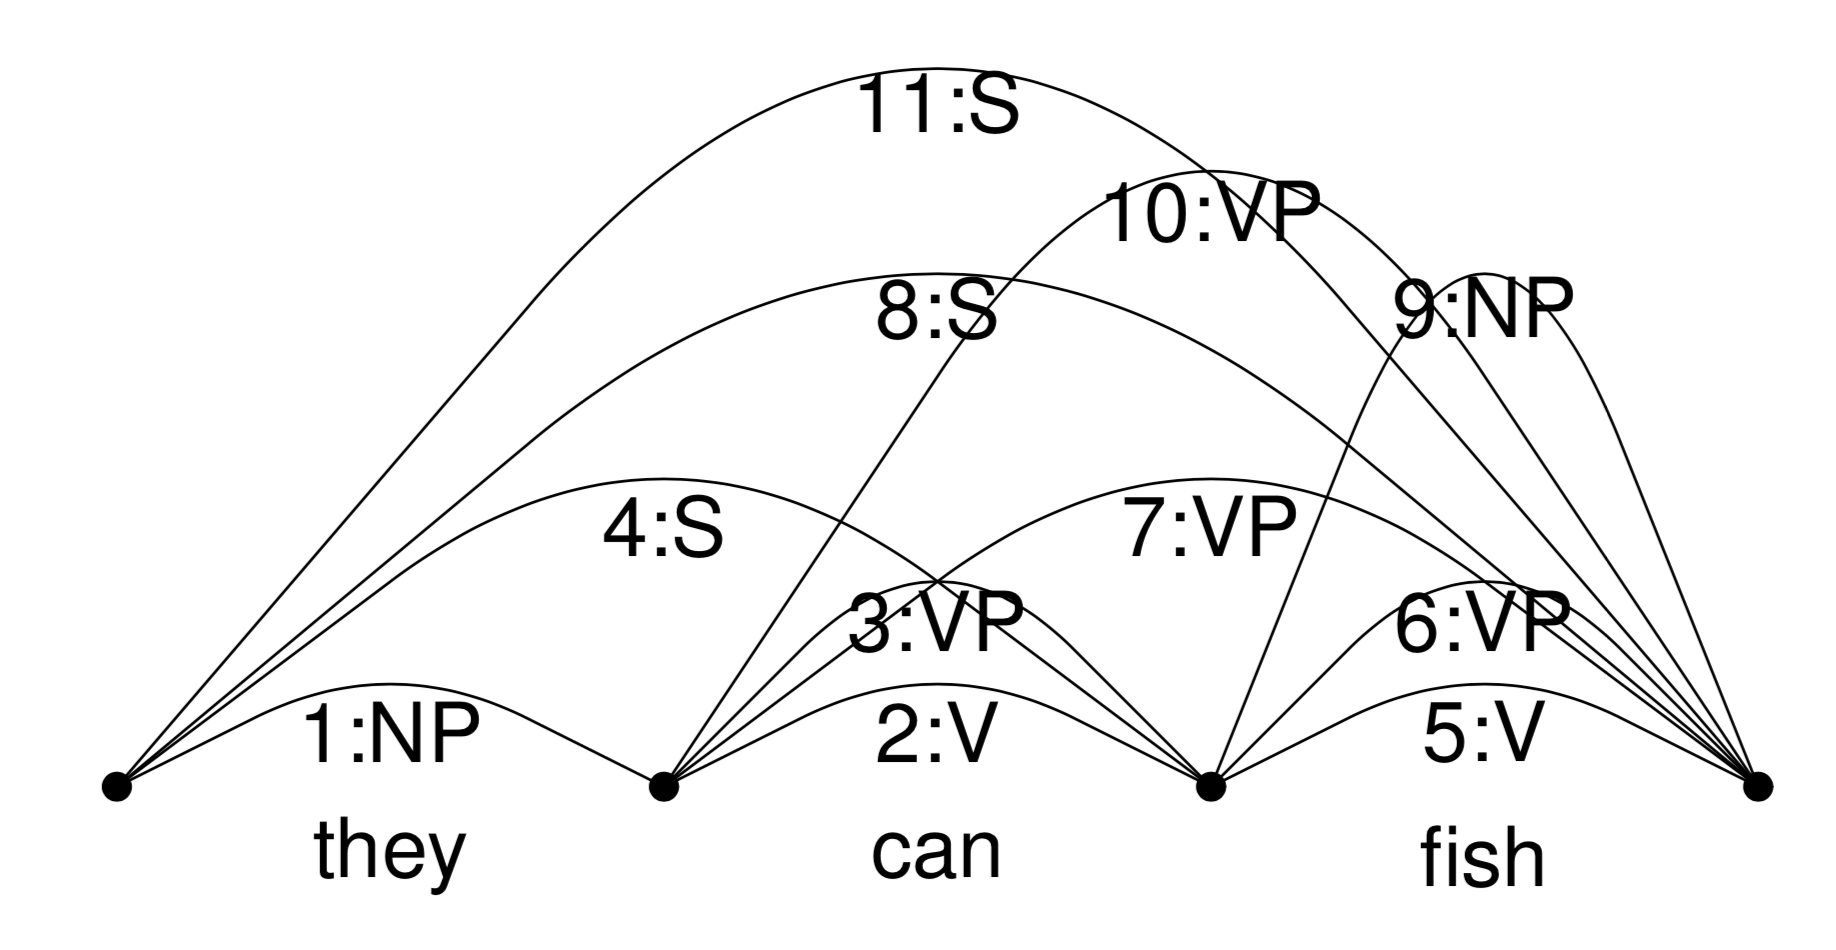
\includegraphics[width=0.5\textwidth]{figures/chart_parsing_structure.png}
		\caption{Example for chart parsing. The resulting chart data structure is shown below.}
		\label{fig:chart_parsing_structure}
	\end{figure}
\end{itemize}
\subsubsection{Implementation of bottom-up parser}
\begin{itemize}
	\item A bottom-up parser would start from the left, look at the first two connections points (first word) and check for a rule that can be applied to this word
	\item If a rule has been found, it is added as edge into the chart, and we start looking for rules that can be applied to the new edge (recursion!). Once no more rule can be applied on this edge and the recursion stops, we go back to the word and continue our search for applicable rules on this word 
	\item After every rule was applied, the parser moves on to the next word on the right and check for rules that can be applied to this word, \textbf{and} all other words/edges that have been processed beforehand. 
	\item Only if no more rules can be applied, the parser moves on to the next word, until all words are processed
	\item The correct parse/grammar structure is this one that end with the start symbol \texttt{S} from the first to the last node of the sentence
	\item Important sub-technique: \textbf{Packing}
	\begin{itemize}
		\item Due to multiple rules with same input, we can have two identical edges that are just based on different daughters
		\item Every following rule is then applied on both edges which is very inefficient
		\item Thus, with \textit{packing} we change the daughter entries to a list of possible daughter lists 
		\item For example, the edge 7 and 10 from the previous example can be combined:
		$$\begin{array}{ccccc}
		\text{id} & \text{left} & \text{right} & \text{mother} & \text{daugthers}\\
		\hline
		7 & 1 & 3 & \texttt{VP} & \left\{\text{(2 6), (2 9)}\right\}\\
		\end{array}$$
		\item If a new daughter list is added, no new recursion/rule application needs to be done  
	\end{itemize}
\end{itemize}
\subsection{Probabilistic parsing}
\begin{itemize}
	\item For a single sentence with 20 or more words, we will get over 1000 analysis $\Rightarrow$ how do we determine the best/most probable analysis?
	\item The traditional approach is it to grammar rules handwritten but they tend to often fail when parsing new sentences
	\item  Current approaches: probabilistic CFG (PCFG) where every rule is augmented with a probability
	\begin{figure}[ht]
		\centering
		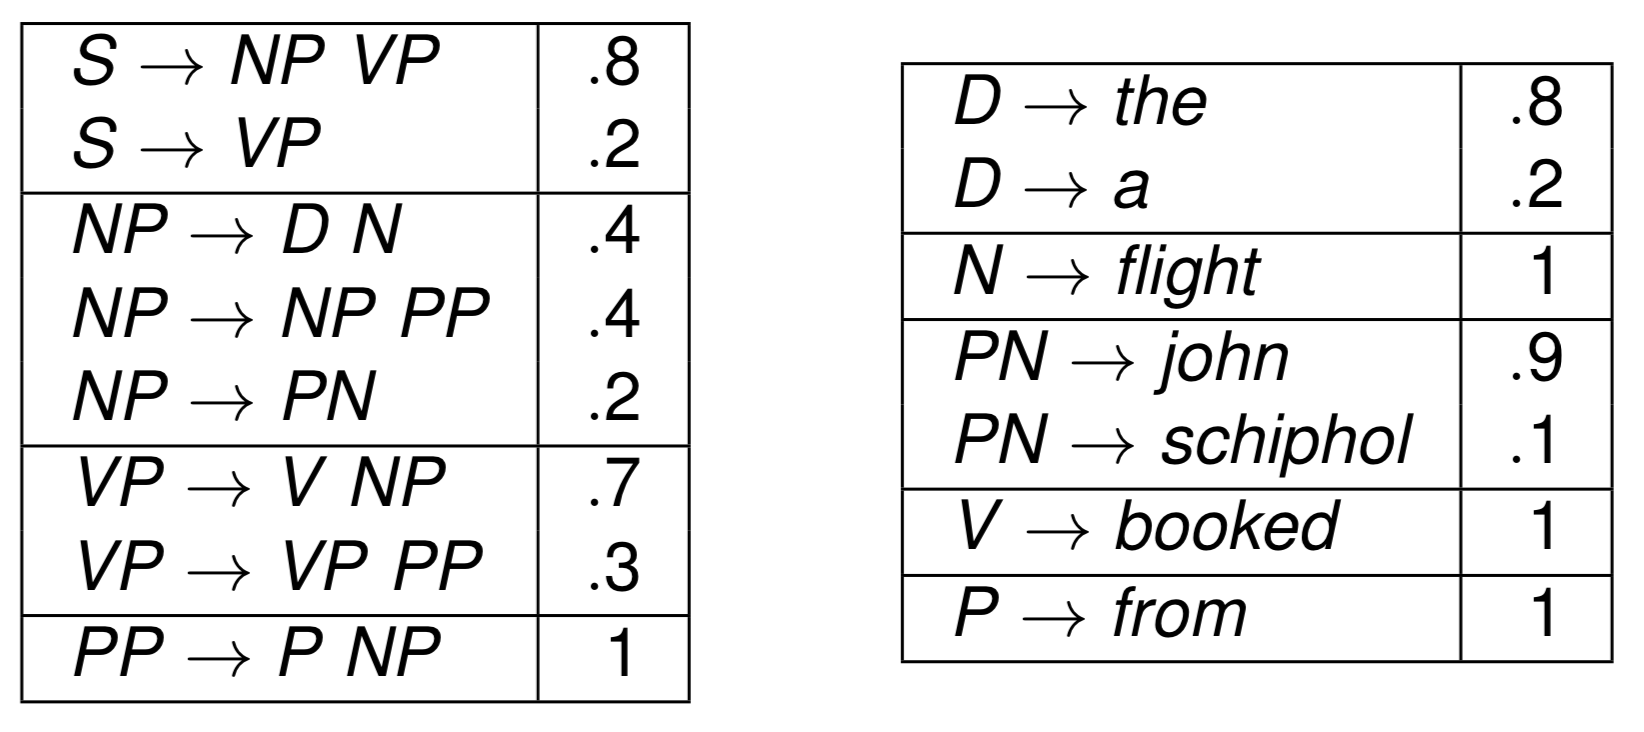
\includegraphics[width=0.35\textwidth]{figures/chart_parsing_prob_cfg.png}
		\caption{Probabilistic CFGs. The probabilities are normalized over all rules with same \textit{left} side.}
		\label{fig:probabilistic_cfg}
	\end{figure}
	\item The probability of a parse tree is the product of the probabilities of all the grammar rules that are used in the sentence derivation
	\item Probabilistic CFGs help for \textit{disambiguation} as we can rank all analysis by probability and just pick the best (n) one(s)
	\item Probabilities can also be used to speed up parsing (drop trees/substructures during parsing that already have a very low probability compared to other current substructures)
\end{itemize}
\subsubsection{Treebank PCFGs}
\begin{itemize}
	\item Instead of specifying/tuning the grammar and its corresponding probabilities by our own, we can use a large dataset of sentences with annotated parse trees
	\item This way, we implicitly get a grammar and the probabilities of each rule
	\item A \textbf{treebank} is therefore a collection of sentences annotated with constituent trees
	\item To estimate the rule probabilities, we use the maximum likelihood:
	$$p(X\to \alpha) = \frac{C(X\to \alpha )}{C(X)}$$
	where $C(X\to \alpha)$ number of times the rule is used in corpus, and $C(X)$ the number of times the non-terminal symbol $X$ appears in treebank
\end{itemize}
\subsubsection{Why CFG and not finite state machines}
\begin{itemize}
	\item Language often has centre-embeddings like $A\to \alpha A \beta$ which cannot be captures by FSAs
	\item However, humans limit the application of such centre-embeddings so that we can convert those into finite rules
	\item The advantage of a FSA would be that we can model hierarchical structures (supported by the fact that we understand the semantic of a sentence, we need good internal structures like the hierarchy)
\end{itemize}
\subsection{Dependency structures}
\begin{itemize}
	\item Context free grammars were based on phrase-structures in sentences
	\item Another possible representation of parsing sentences is using directed/asymmetric binary grammatical relations that hold among the words 
	\item A relation consists of 
	\begin{itemize}
		\item a head \texttt{H} (central word)
		\item a dependent \texttt{D}
		\item a label identifying the relation between \texttt{H} and \texttt{D}
	\end{itemize}
	\begin{figure}[ht]
		\centering
		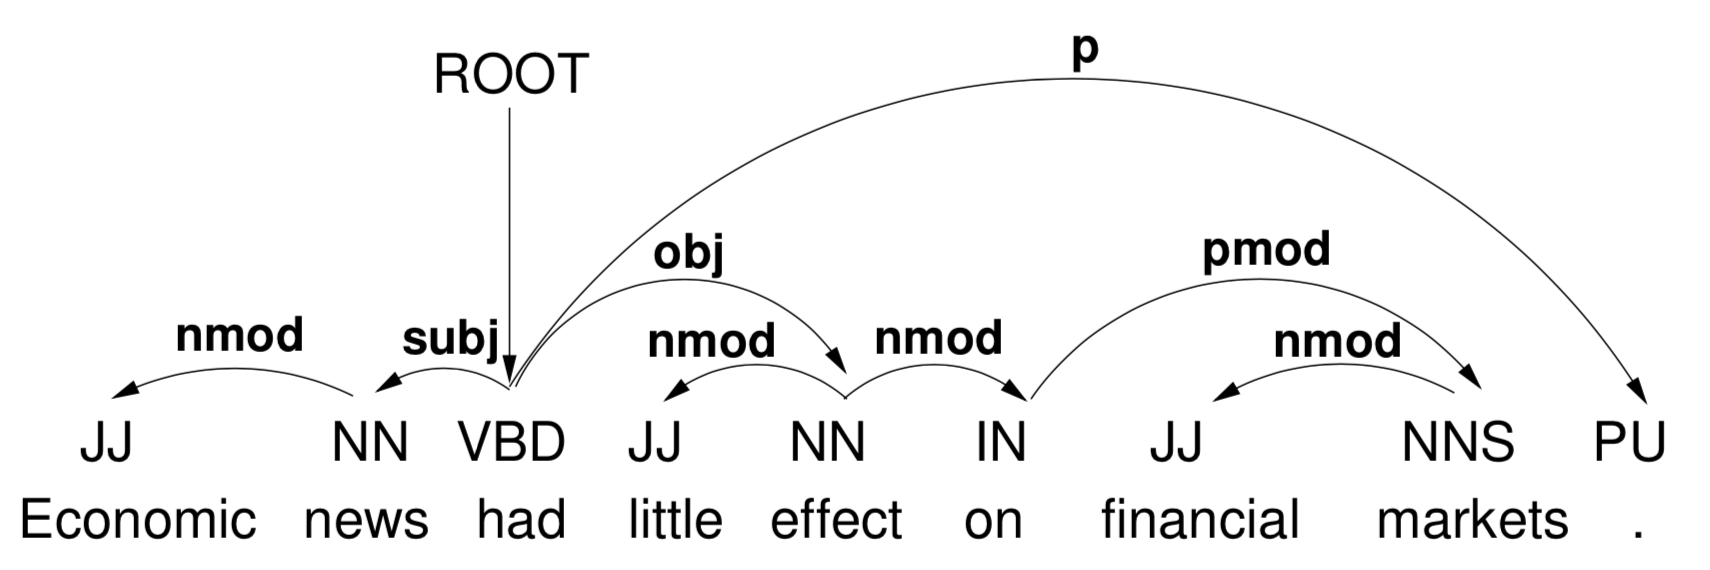
\includegraphics[width=0.5\textwidth]{figures/dependency_parsing.png}
		\caption{Dependency parsing. All relations are directed form head \texttt{H} to dependent \texttt{D}.}
		\label{fig:dependency_parsing}
	\end{figure}
	\item It is important to prevent parsing errors as these can significantly change the semantic of a sentence
\end{itemize}
\section{Lexical and distributional semantics}
\begin{itemize}
	\item \textbf{Compositional semantics}: meaning of phrase/sentence
	\item \textbf{Lexical semantics}: meaning of individual words
\end{itemize}
\subsection{Approaches for lexical meaning}
\begin{itemize}
	\item How to represent a meaning of a word. Problem: no representation can fully capture language yet!
\end{itemize}
\subsubsection{Formal semantics}
\begin{itemize}
	\item Based on set theory, describing the features of a word
	\item Meaning postulates: $\forall x \left[\text{bachelor}'(x)\to\text{man}'(x)\wedge\text{unmarried}'(x)\right]$
	\begin{itemize}
		\item If a word is in the set \textit{bachelor}, then it also is in \textit{man} and \textit{unmarried}
	\end{itemize}
	\item Problems:
	\begin{itemize}
		\item Limited, especially for special cases (i.e. what is the Pope?)
		\item Very expensive for large corpus
		\item For some words, it is almost impossible to find a good formalization
	\end{itemize}
	\item Alternative: \textbf{Prototype theory}
	\begin{itemize}
		\item Notion of graded semantic categories with no clear boundaries
		\item No requirement that a feature must be shared by all members
		\item Certain members are more central or prototypical $\Rightarrow$ \textbf{Protoypes}
		\item New members are added based on similarity to prototypes
		\item Features and category memberships are graded
	\end{itemize}
\end{itemize}
\subsubsection{Semantic relations}
\begin{itemize}
	\item \textbf{Hyponymy}: IS-A relation, forms a taxonomy (\textit{Example}: dog is a hyponym of animal)
	\begin{itemize}
		\item Easier to construct for certain nouns, but especially hard for adjectives
	\end{itemize}
	\item \textbf{Meronomy}: PART-OF relation (\textit{Example}: arm is a meronym of body)
	\item \textbf{Synonymy}: Words can be exchanged without changing the meaning of a sentence/phrase
	\item \textbf{Antonymy}: Opposite meanings (\textit{Example}: big vs. little)
\end{itemize}
\subsubsection{WordNet}
\begin{itemize}
	\item Large-scale corpus for English resource
	\item Handconstructed
	\item Organized in synsets: sets of synonyms
	\item Synsets are connected by semantic relations
	\item Similarity of words is the similarity of synsets
\end{itemize}

\subsection{Polysemy and word sense disambiguation}
\begin{itemize}
	\item A word can mean different things based on the sentence/context it is used in
	\item Meaning of words is not fixed, but dynamically adapted by the context
	\item \textbf{Regular polysemy}: mechanisms to apply on words to fit into context
	\begin{itemize}
		\item \textit{Zero-derivation}: verb $\leftrightarrow$ noun without changing word. Example: ``\textit{tango}''
		\item \textit{Metaphorical}: using words from a different domain to express similar meaning. Example: ``\textit{swallow information}''
		\item \textit{Metonymy}: use an entity to actually refer to other aspects of it. 
		Example: ``\textit{drinking his glass}''
	\end{itemize}
	\item \textbf{Word sense disambiguation}: derive meaning of word in context
	\begin{itemize}
		\item \textit{Supervised} (most common) $\to$ predefined list of senses (i.e. WordNet), and train model on \textit{large} corpus. Problem: we have to learn a new classifier for every word!
		\item \textit{Semi-supervised} $\to$ annotate small dataset, bootstrap from there. Might be helpful as some instances have no single/discrete meaning.
		\item \textit{Unsupervised} $\to$ induce sense by clustering of word occurences. Usually, the result is either too fine-grained or coarse-grained for most word (only work great for frequent words)
	\end{itemize}
\end{itemize}
\subsubsection{Semi-Supervised WSD: Yarowsky algorithm}
\begin{itemize}
	\item Using bootstrapping which needs only a very small hand-labeled training set
	\item Still, learns a classifier for every word $\Rightarrow$ no generalization!
	\item Also, define features (see notion of context) for every word to determine its meaning
	\item \textbf{Algorithm iteration}: 
	\begin{enumerate}[start=0]
		\item Given a small initial seed set $\Lambda_0$ of labeled instances of each sense, and a much larger unlabeled corpus $V_0$
		\item Train classifier on $\Lambda_0$
		\item Use trained classifier to label $V_0$
		\item Select the examples in $V_0$ that the classifier is most confident on
		\begin{enumerate}
			\item Reliability of a prediction defined as $\log\left(\frac{p(a|w)}{p(b|w)}\right)$ for word w and possible senses $a$ and $b$
			\item Rank reliabilities of all predictions and choose $n$ best
		\end{enumerate}
		\item Remove chosen examples from $V_0\Rightarrow V_1$, and add them to the training set $\Rightarrow\Lambda_1$
		\item Repeat step 2) to 4) until:
		\begin{enumerate}
			\item Either $V_i$ is empty
			\item Or the error rate on the training/validation is sufficient low
		\end{enumerate}
	\end{enumerate}
	\item Reported accuracy of 95\%, but on easy homonymous examples
	\item \textbf{One sense per discourse}
	\begin{itemize}
		\item Original algorithm uses \textit{one sense per discourse} as second heuristic
		\item If a word appears twice or more often in the same text, they are probably of the same meaning\\
		$\Rightarrow$ Annotate these as well and use them as additional training examples
	\end{itemize}
\end{itemize}
\subsection{Distributional semantics}
\begin{itemize}
	\item Probabilistic models for semantics
	\item Distributional hypothesis about word meaning: the meaning of a word is determined by its context $\Rightarrow$ similar meanings have similar contexts
	\item Thus, distributions are a good conceptual representation if you believe that ‘the meaning of a word is given by its usage’ $\Rightarrow$ Corpus-dependent like different culture, domains, ...
	\item Distributions can encode lexical- and world knowledge, but mostly only partial lexical semantics 
	\item Techniques: Count-based models and prediction models
\end{itemize}
\subsubsection{Count-based models}
\begin{itemize}
	\item Vector spaced models in the semantic space, where every dimension corresponds to a possible context $\Rightarrow$ features
	\item Distribution can be seen as point in space
	\item As a result, we get a feature matrix:
	$$\begin{array}{c|cccc}
	& \text{feature}_1 & \text{feature}_2 & \dots & \text{feature}_n\\
	\hline
	\text{word}_1  & f_{1,1} & f_{2,1} & \dots & f_{n,1}\\
	\text{word}_2  & f_{1,2} & f_{2,2} & \dots & f_{n,2}\\
	\vdots  & \vdots & \vdots & \ddots & \vdots\\
	\text{word}_m  & f_{1,m} & f_{2,m} & \dots & f_{n,m}\\
	\end{array}$$
	\item Possible design choices in count-based models:
\end{itemize}
\begin{enumerate}
	\item \textbf{Notion of context}: how to define the context of a word
	\begin{enumerate}
		\item \textit{Word windows}: n words on either side of the lexical item, and count occurrences of words
		\item \textit{Filtered word windows}: n words, but remove irrelevant words based on POS-tag or stop-list (don't need to extend window)
		\item \textit{Lexeme windowing}: word windows (filtered or unfiltered), but with using stemming (mostly lead to more robust models)
		\item \textit{(Syntactic) dependencies}: context with dependency structure it belongs to (directed link between heads and dependents). Can be used with different extends\\
		Example: ``The prime minister acknowledged the question'' \\
		- [prime\_a 1, acknowledge\_v 1] (a for adjectives, v for verbs)\\
		- [prime\_a\_mod 1, acknowledge\_v\_subj 1] (mod for modifiers, subj for verb in relation to subject)\\
		$\Rightarrow$ Problem: complex context lead to sparse vectors
	\end{enumerate}
	$\Rightarrow$ Working best: small window sizes or short dependencies
	\item \textbf{Context weighting}: how to set the weights in the vector
	\begin{enumerate}
		\item \textit{Binary model}: if $c$ co-occurs with word $w$, value of entry is 1, else 0
		\item \textit{Basic frequency model}: number of times $c$ co-occurs (probably normalized)
		\item \textit{Characteristic model}: weights express how characteristic a given context is for a word $w$\\
		\item \textit{Pointwise Mutual Information (PMI)}: example of characteristic model. Comparing probability of both words occur together compared to occurring alone.\\
		$$PMI(w,c)=\log \frac{P(w,c)}{P(w)P(c)} = \log \frac{P(c|w)}{P(c)} \text{\hspace{5mm} where \hspace{5mm}}P(c) = \frac{f(c)}{\sum_k f(c_k)}, P(c|w) = \frac{f(w,c)}{f(w)}$$
		$$\Rightarrow PMI(w,c) = \log \frac{f(w,c)\sum_k f(c_k)}{f(w)f(c)}$$
		$PPMI\to$ only use positive values, $PPMI(w,c) =\max\left(PMI(w,c),0\right)$
	\end{enumerate}
	\item \textbf{Semantic space}: what are possible contexts
	\begin{enumerate}
		\item \textit{Entire vocabulary}: every word represents a possible context.\\
		+ All info included (also the rare one) - Inefficient (large space \& sparse), noisy
		\item \textit{Top n words with highest frequency}: \\
		+ More efficient, noise is filtered out - May miss out infrequent contexts
		\item \textit{Singular Value Decomposition}: dimension reduction by exploiting redundancies\\
		+ Very efficient, good generalization - Not interpretable (or very hard)
		\item \textit{Non-negative matrix factorization}: Similar to SVB, but performs factorization differently
	\end{enumerate}
\end{enumerate}
\subsubsection{Prediction-based models}
\begin{itemize}
	\item Train a model to predict plausible contexts for a word
	\item Learn word representations in the training process
	\item \textbf{Short dense} embeddings with \textbf{latent} dimensions 
	\begin{itemize}
		\item Easier to use as features with machine learning
		\item Better generalization than simple counting $\Rightarrow$ capturing more complex relations like synonym
	\end{itemize}
	\item One example for prediction-based models is skip-gram, also known as word2vec (see later section)
\end{itemize}
\subsubsection{Similarity}
\begin{itemize}
	\item Definition of similarity very broad. Can include synonym, antonyms, hyponyms, ...
	\item Measuring similarity with \textbf{Cosine} between vectors $v$ and $u$:
	$$\cos\left(\theta\right) = \frac{\sum_k v_k \cdot u_k}{\sqrt{\sum_k v_k^2} \cdot \sqrt{\sum_k u_k^2}}$$
	\item Cosine measure calculates the angle between $v$ and $u$, and is length-independent (normalization). Important as frequent words can have longer vectors
	\item Other measures include Jaccard, Euclidean distance (vectors need to be normalized!), ...
	\item However, true-synonyms do not always get higher similarity scores than near-synonyms, and also to antonyms
	\item Identifying antonyms by extra heuristics like checking words with high similarity that frequently appear together (\textit{example}: ``we serve hot and cold drinks'')
	
\end{itemize}
\subsubsection{Distributional word clustering}
\begin{itemize}
	\item Cluster words based on the contexts they occur
	\item Predefine number of clusters and corpus (for instance 2000 nouns in 200 clusters)
	\item \textbf{Features} can represent different kinds of contexts
	\begin{itemize}
		\item Windows based context, parsed or unparsed, syntactic dependencies
		\item Define notion of context, context weighting, and semantic space 
		\item Feature representation can significantly influence performance
	\end{itemize}
	\item Clustering algorithm: K-means
	\begin{itemize}
		\item Given dataset with $N$ points and task of $K$ clusters, minimize sum of squares of distance of each data point to its closest cluster mean $\bm{\mu}_i$:
		$$\arg\min_C \sum\limits_{i=1}^{K}\sum\limits_{\bm{x}\in C_i} ||\bm{x} - \bm{\mu}_{i}||^2$$
	\end{itemize}
	\item Small context sizes (small windows, syntactic dependencies) lead to clusters of synonyms (words that can be replaced)
	\item Large context sizes lead to \textbf{topical similarity} (words belonging to the same topic)
\end{itemize}

\subsubsection{Skip-gram}
\begin{itemize}
	\item Sometimes referred to as \textit{word2vec} because it is implemented in this package
	\item Given a word $w_t$, predict neighbouring words in a context windows of $2L$ words (for $L=2$: $w_{t-2}, w_{t-1}, w_{t+1}, w_{t+2}$) 
	\item In skip-gram, we learn two representations for every word $w_j \in V$:
	\begin{itemize}
		\item \textbf{word embedding} $v$ in word matrix $W$
		\item \textbf{context embedding} $c$ in context matrix $C$ (word in the role as context for other words)
	\end{itemize}
	\item To learn these embeddings, we take every word $w(t)$ in the corpus (index $j$ in vocabulary), and try to predict $w(t+1), ...$ where we denote this word with index $k$ in the vocabulary: 
	$$p\left(w_k | w_j\right)$$
	\item The idea in skip-gram is that we compute this probability by the similarity between the words $w_k$ and $w_j$ whereas we use the context matrix $C$ for $w_k$ and the word matrix $W$ for $w_j$ (see figure below)
	\begin{figure}[ht]
		\centering
		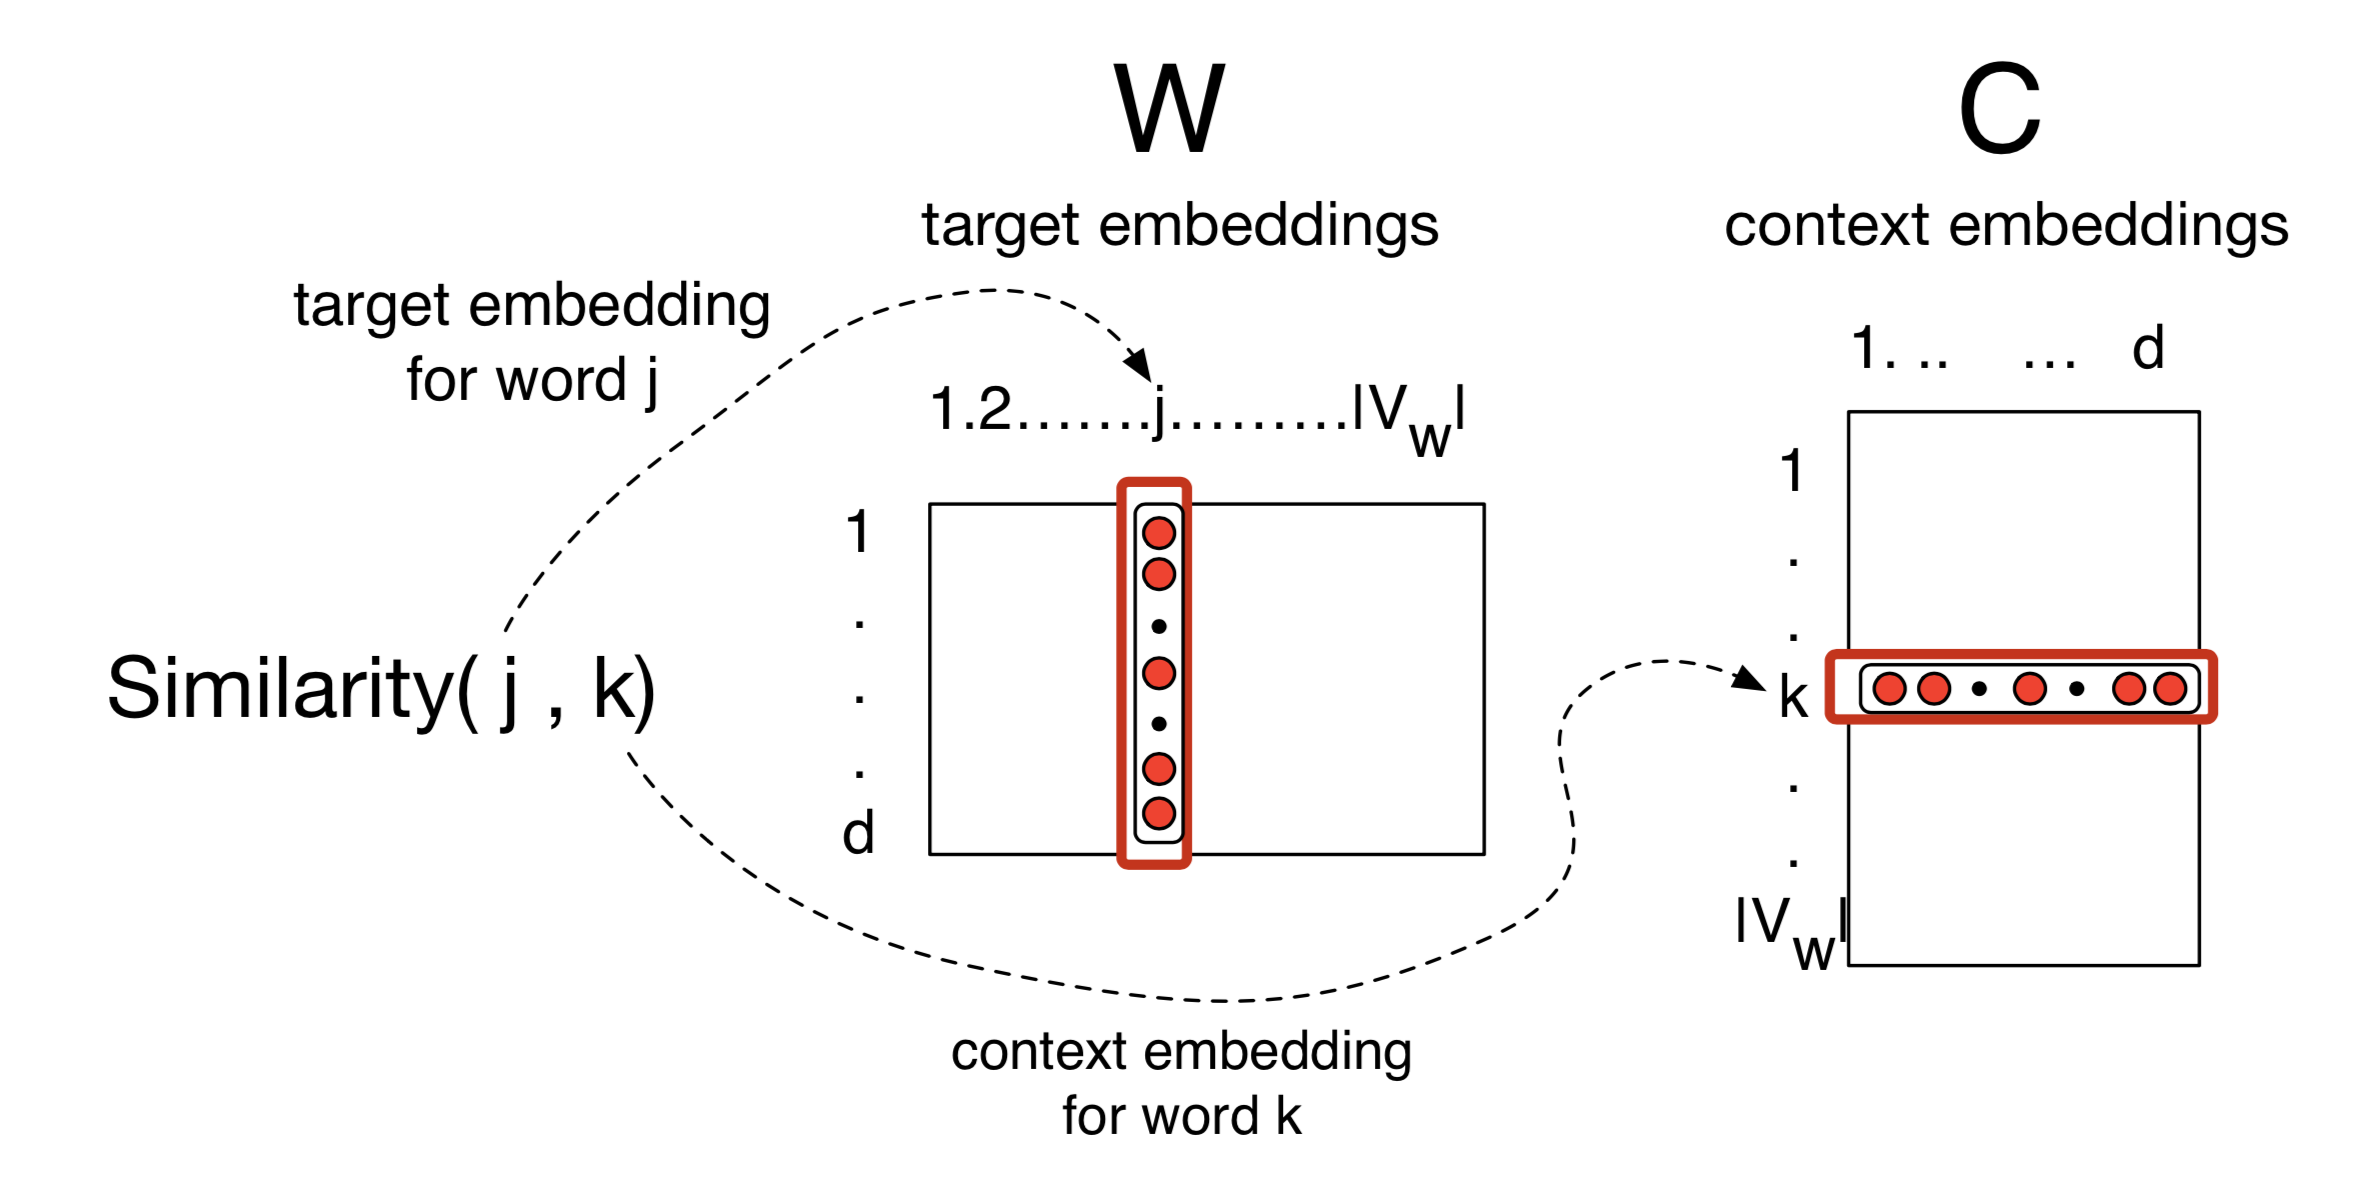
\includegraphics[width=0.5\textwidth]{figures/skip_gram_matrices.png}
		\caption{Skip gram overview}
		\label{fig:skip_gram_matrices}
	\end{figure}
	\item Similar to the cosine similarity, we use the dot product for calculating this:
	$$\text{Similarity}(c_k, v_j)\propto c_k\cdot v_j$$
	\item To normalize and get probability distribution over contexts, we use the softmax function:
	$$p\left(w_k|w_j\right)=\frac{\exp\left(c_k \cdot v_j\right)}{\sum_{i\in V} \exp\left(c_i \cdot v_j\right)}$$
	\item For the learning process, we start with randomly initialized vectors, and try to maximize the log-likelihood of the dataset (by performing SGD or similar):
	$$\arg\max \sum\limits_{\left(w_j, w_k\right)\in D} \log p\left(w_k|w_j\right) = \sum\limits_{\left(w_j, w_k\right)\in D}  \left(c_k \cdot v_j - \log \sum\limits_{c_i \in V} \exp\left(c_i \cdot v_j\right)\right)$$
	\item We can also represent skip-gram as a (neural) network:
	\begin{figure}[ht]
		\centering
		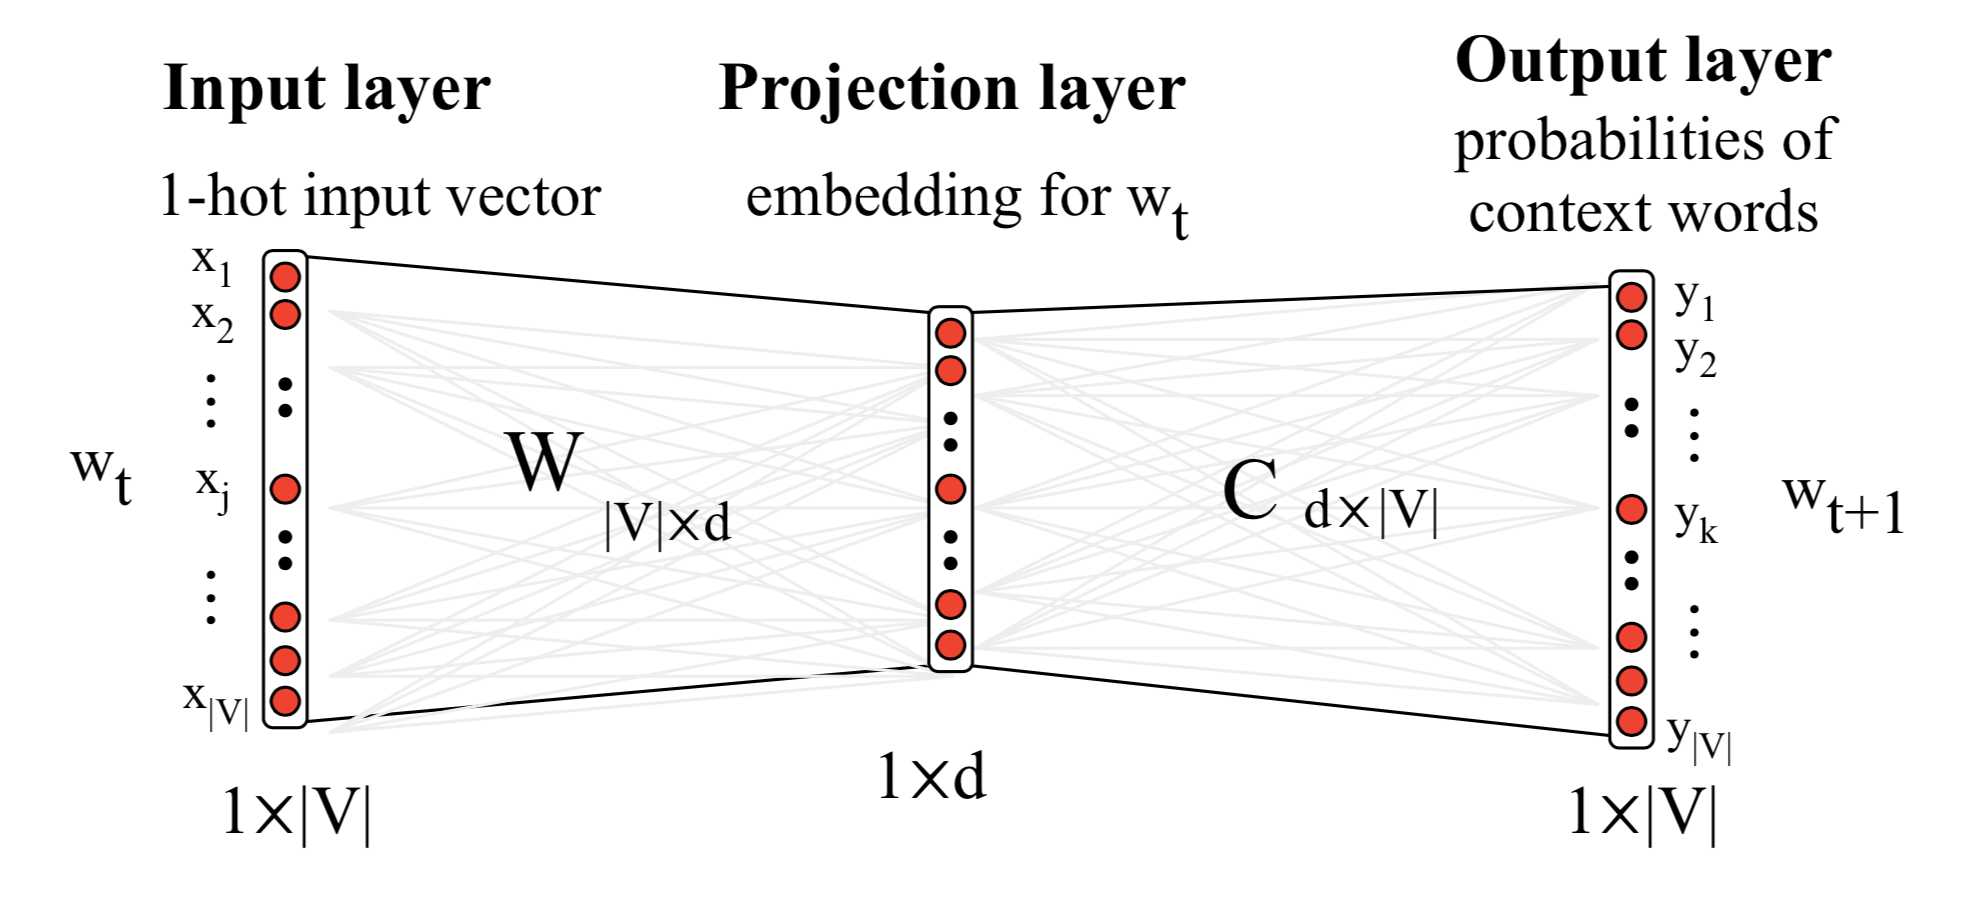
\includegraphics[width=0.5\textwidth]{figures/skip_gram_nn.png}
		\caption{Skip gram as neural network. The weights of the first layer represent the word embedding $W$, whereas the context embedding $C$ is in the second layer.}
		\label{fig:skip_gram_nn}
	\end{figure}
	\item However, the problem here is that for a large vocabulary size, the denominator of the softmax is very expensive to calculate $\Rightarrow$ \textbf{negative sampling}
	\begin{itemize}
		\item Approximate denominator by sampling $k$ random words from vocabulary (probability of sampling for a word is mostly connected to its unigram probability/frequency in the corpus like $\text{count}^{\alpha}(w)$ with for example $\alpha=0.75$)
		\item Dataset consists therefore out of words pair which are either positive or negative examples for context + word (note that we do not distinguish between the probability calculation of $w_{t-2}$ and $w_{t-1}$ for example)
		\item We convert the classification task into predicting whether a context pair is a positive or negative example from the corpus
		$$p\left(+|w_j, w_k\right) = \sigma(c_k\cdot v_j) = \frac{1}{1 + \exp(-c_k\cdot v_j)}$$
		$$p\left(-|w_j, w_k\right) = 1 - p\left(+|w_j, w_k\right) = \frac{1}{1 + \exp(c_k\cdot v_j)}$$
		$$\Rightarrow \arg\max \sum\limits_{\left(w_j, w_k\right)\in D_{+}} \log p\left(+|w_k,w_j\right) + \sum\limits_{\left(w_j, w_k\right)\in D_{-}} \log p\left(-|w_k,w_j\right) $$
	\end{itemize}
	\item Embeddings capture \textbf{analogies}: \textit{a} is to \textit{b} as \textit{c} is to \textit{d}
	\begin{itemize}
		\item Due to similarity, we can use the offsets to find the appropriate word $d$:
		$$a-b\approx c-d \Rightarrow d' = \arg\max_{d'_w \in V} \cos\left(a-b, c-d'\right)$$
	\end{itemize}
	\item Word2vec is often used as initialization/pretraining for other tasks. Reasons:
	\begin{itemize}
		\item Will help the model to start from an informed position
		\item Only needs a plain text corpus without any annotation
		\item Is very fast and pretrained versions are also available on the internet
		\item Best performance can be achieved by fine-tuning the weights afterwards
	\end{itemize}
\end{itemize}
\section{Compositional semantics and discourse processing}
% \subsection{Compositional semantics}
\begin{itemize}
	\item \textbf{Principle of Compositionality}: meaning of whole phrase derivable from meaning of its parts
	\item Sentence structure conveys some meaning as well
	\begin{itemize}
		\item Different syntactic structures may have the same meaning, but similar syntactic structures can also have different meanings
	\end{itemize}
	\item Not all phrases are interpreted compositionally (e.g. \textit{kick the bucket}) but can be grouped together and viewed as one element
	\item Meaning of a single word can depend on the composition (\textit{fast} programmer vs. \textit{fast} plane, metaphors,...)
\end{itemize}
\subsection{Compositional distributional semantics}
\begin{itemize}
	\item Extending distributional semantics to phrases/sentences
	\item Unsupervised model $\Rightarrow$ general-purpose representations
	\item Model composition in vector space. However, if we would model every sentence as independent, we would get an infinite dimensional space
\end{itemize}
\subsubsection{Vector mixture model}
\begin{itemize}
	\item Combining the vectors of all words in the sentence
	\item Mostly done either additive (adding all vector) or multiplicative (elementwise product of vectors)
	\item Problem: does not consider word order and is therefore suitable for modelling content words (nouns, verbs, adjectives,...), but not for function words that require syntactic dependencies (pronouns, ...)
	\item Is often used as baseline
\end{itemize}
\begin{figure}[ht]
	\centering
	\begin{subfigure}{0.3\textwidth}
		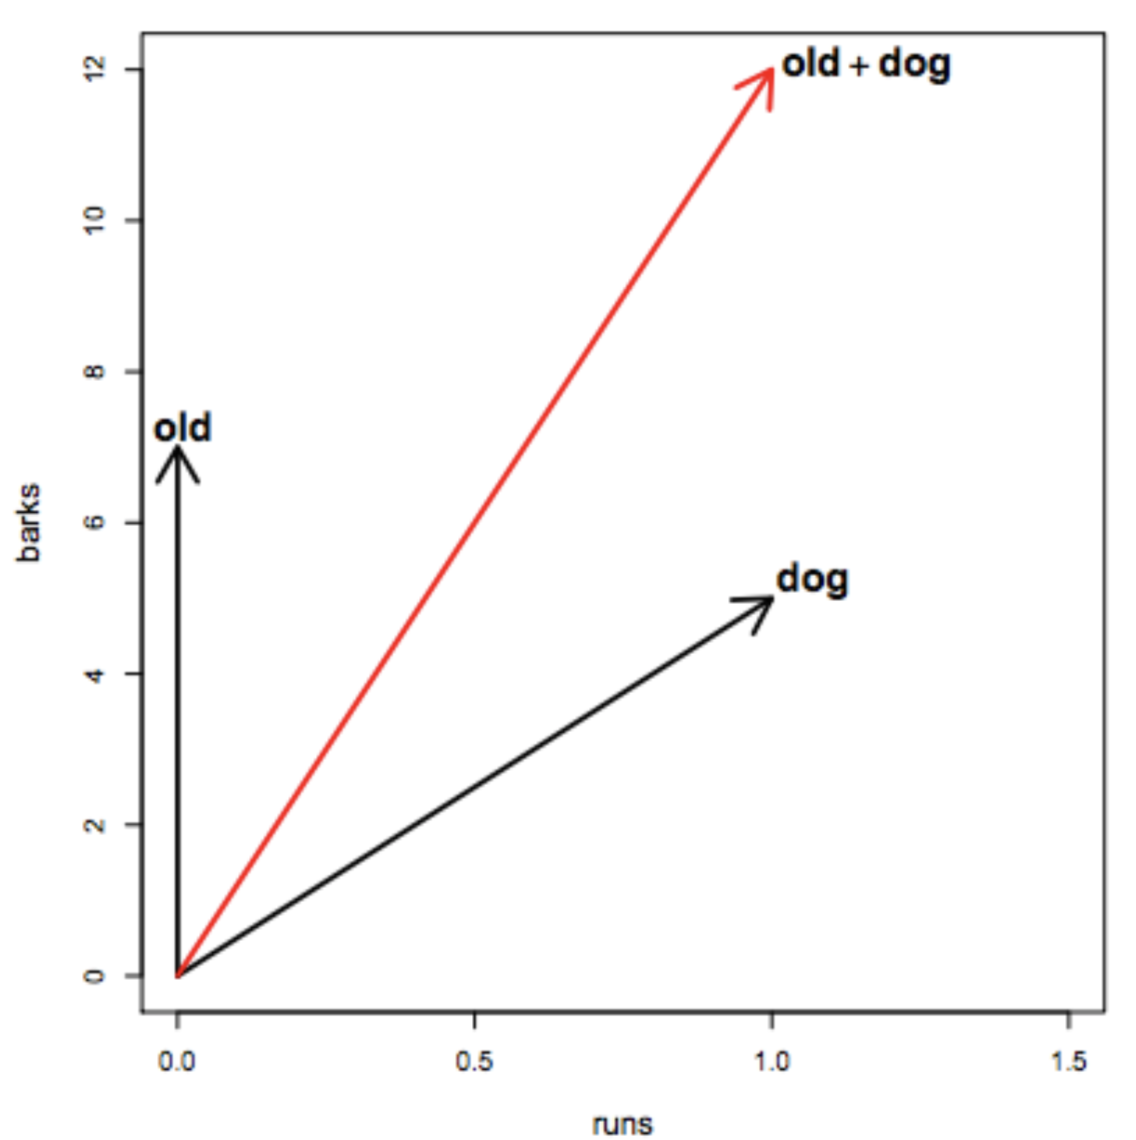
\includegraphics[width=\textwidth]{figures/compositional_semantic_vector_mixture_model.png}
		\caption{Vector mixture model}
	\end{subfigure}
	\begin{subfigure}{0.3\textwidth}
		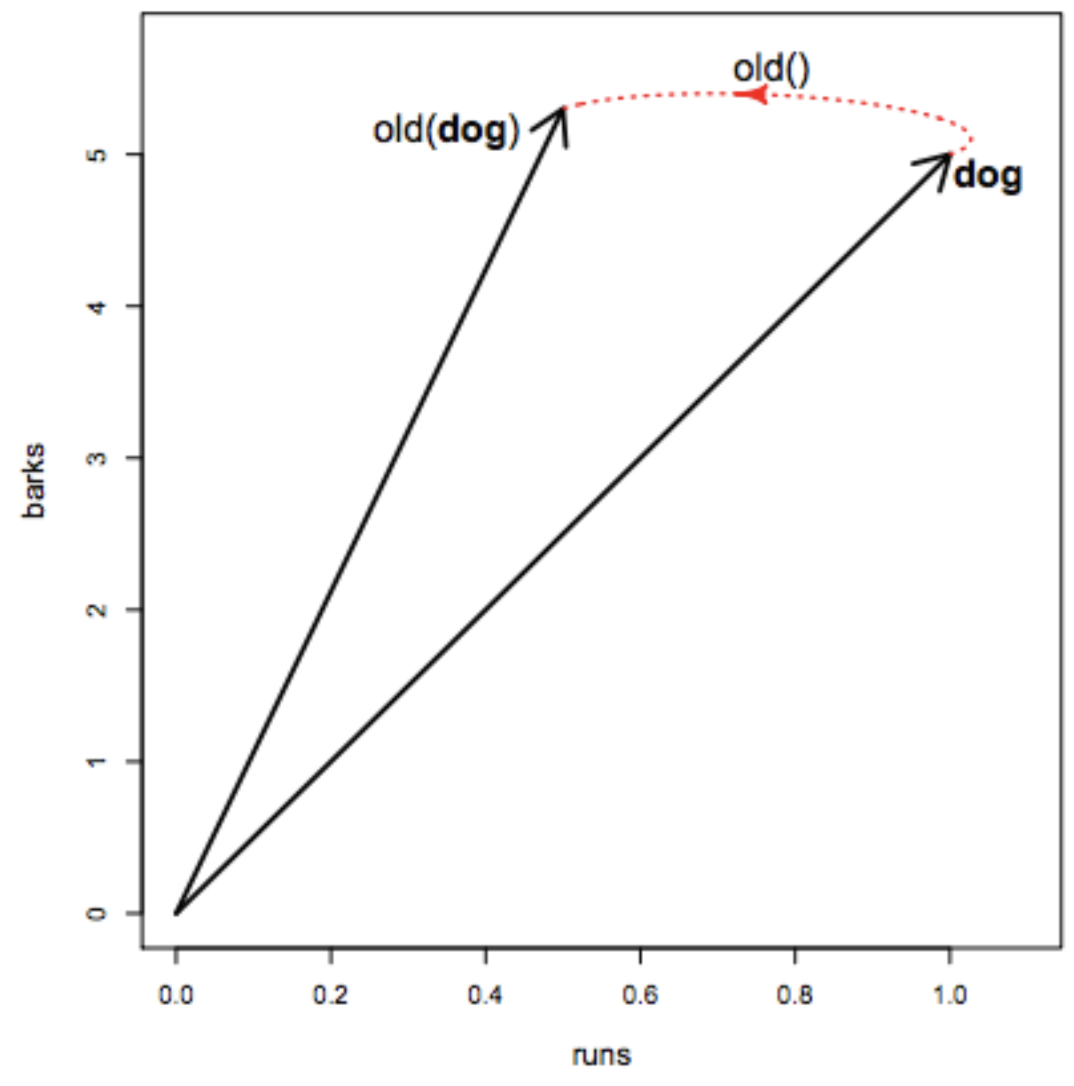
\includegraphics[width=\textwidth]{figures/compositional_semantics_lexical_function_models.png}
		\caption{Lexical function model}
	\end{subfigure}
	\caption{Compositional distributional semantics}
	\label{fig:compositional_semantic_vector_mixture_model}
\end{figure}
\subsubsection{Lexical function model}
\begin{itemize}
	\item Discriminate between words that meaning is determined by its context/distribution (e.g. nouns), and function words that are applied on the represented words as \textbf{lexical functions}
	\item Example: $\underbrace{\textit{old}}_{\text{functional}} \underbrace{\textit{dog}}_{\text{distributional}} \Rightarrow$ apply function of \textit{old} on \textit{dog}
	\item Lexical functions are parameter matrices (i.e. $\bm{A}_{\textit{old}}$) which are multiplied with the vector representation of nouns
	\begin{figure}[ht]
		\centering
		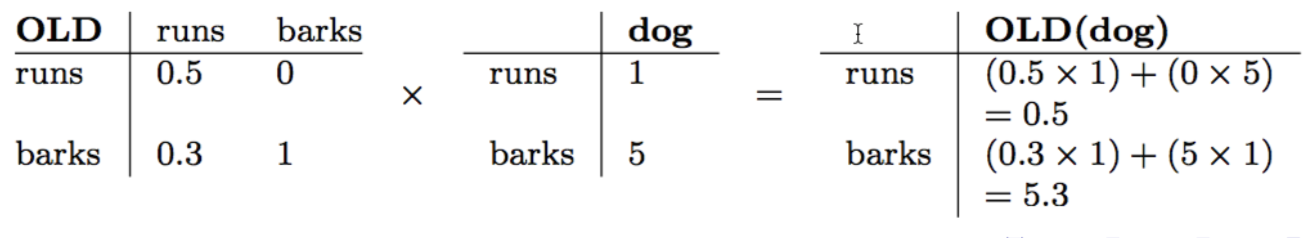
\includegraphics[width=0.5\textwidth]{figures/compositional_semantics_lexical_function_models_adjectives.png}
	\end{figure}
	\item Adjectives that does not change the meaning of a word are diagonal up to identity matrix $\Rightarrow$ element captures how features interact with each other given the adjective
	\item The matrices are learned by comparing the representation of plain nouns to combination of noun and adjective. Pseudo-code algorithm:
	\begin{enumerate}
		\item Obtain a distributional vector $n_j$ for each noun $n_j$ in the lexicon.
		\item Collect adjective noun pairs $(a_i,n_j)$ from the corpus.
		\item Obtain a distributional vector $p_{ij}$ of each pair $(a_i,n_j)$ from the same corpus using a conventional DSM.
		\item The set of tuples $\{(n_j,p_{ij})\}_j$ represents a dataset $\mathcal{D}(a_i)$ for the adjective $a_i$.
		\item Learn matrix $\bm{A}_i$ from $\mathcal{D}(a_i)$ using linear regression by minimizing:
		$$L(\bm{A}_i) = \sum\limits_{j\in \mathcal{D}(a_i)} ||p_{ij} - \bm{A}_i n_j||^2$$
	\end{enumerate} 
	\item Verbs can be represented as high-order tensors. If only subject is taken into consideration, it is a two-dimensional matrix. When also considering object, then it is three dimensional (or even higher)
	\item \textit{Polysemy} (different forms of a word) are mostly handled by a single representation. We assume that ambiguity can be handled as long as the context is given.
	\item To identify \textit{metaphors}, two separate senses of every adjective can be learned (literal and metaphorical). We then map from literal to metaphorical by a linear transformation. 
\end{itemize}
\subsubsection{Compositional semantics in neural networks}
\begin{itemize}
	\item Supervised learning framework $\Rightarrow$ compositional representations are fine-tuned for specific application/task
	\item Word representations are taken as input and processed within the network
	\item Example tasks include sentiment classification, paraphrasing, machine translation, ...
	\item Using recurrent and/or recursive networks (LSTMs, Tree-LSTMs, ...)
\end{itemize}
\subsection{Discourse structure}
\begin{itemize}
	\item Most documents have a implicit (in news paper articles, first sentence is a summary) or explicit structure like sections and paragraphs
	\item There are also relationships between sentences that need to be modeled as follow
\end{itemize}
\subsubsection{Rethorical relations}
\begin{itemize}
	\item There are implicit relations between sentences. For example:\\
	\texttt{Max fell. John pushed him.}\\
	can be interpreted as \textit{explanation} (Max fell because John pushed him), or as \textit{narration} (Max fell and then John pushed him).
	\item This relation is called \textbf{discourse relation} or \textbf{rhetorical relation}
	\item \textbf{Cue phrases} indicate what kind of relation it is. In the previous examples, the cue phrases were \texttt{because} and \texttt{and then}.
	\item Analyzing a text for rhetorical relations mostly gives a binary structure: the main sentence is called \textbf{nucleus}, and subsidiary phrase (explanation, justification, ...) is called \textbf{satellite}
	\item In a \textit{narration} (cue phrase \texttt{and}) both sentences have equal weight instead of nucleus vs satellite.
\end{itemize}
\subsubsection{Coherence}
\begin{itemize}
	\item Discourses need to have connectivity/context to be coherent.
	\item Otherwise, a sentence/small discourse might not make sense
	\item However, this information is mostly missing (background/world knowledge)!
	\item Assuming discourse coherence can affect interpretation. Especially when dealing with pronouns, th
\end{itemize}
\subsubsection{Overview of factors influencing discourse interpretation}
\begin{enumerate}
	\item \textit{Cue phrases} (\texttt{because}, \texttt{and}, ...)
	\item \textit{Punctuation and text structure} (\texttt{Max fell (John pushed him), and Kim laughed.})
	\item \textit{Real world context} (\texttt{Max was falling.} \texttt{John pushed him as he lay on the ground.})
	\item \textit{Tense and aspects} (\texttt{Max was falling.} \texttt{John pushed him.})
\end{enumerate}
\begin{itemize}
	\item Discourse parsing (understanding discourse structure) is a hard task
	\item Mostly done by supervision (annotated data of about 8-10 discourses)
	\item However, \textit{surface techniques} (primitive algorithms that look at characteristic phrases, punctuation, ...) seem to work to some extent
\end{itemize}
\subsection{Referring expressions and anaphora}
\begin{itemize}
	\item To fully process a discourse, co-references/referring expressions like pronouns need to be resolved
	\item We can define the following entities for a referring expression:
	\begin{itemize}
		\item \textit{referent} - a real world entity to which is referred
		\item \textit{referring expression} - part of speech that refers to an entity
		\item \textit{antecedent} - the text initially evoking a referent (where referent is named)
		\item \textit{anaphora} - the phenomenon of referring to an antecedent
		\item \textit{cataphora} - pronouns that appear \textit{before} the pronoun (rare)
	\end{itemize}
	\item \textbf{Pronoun resolution}
	\begin{itemize}
		\item Identifying the referents of pronouns
		\item \textit{Anaphora resolution}: in most cases, the task is limited to identifying referents that are mentioned before the actual pronoun/reference
	\end{itemize}
\end{itemize}
\subsubsection{Algorithms for anaphora resolution}
\begin{itemize}
	\item For anaphora resolution, we mostly apply a supervised training algorithm
	\item The instances in the corpus are possible pairs of pronoun and antecedent (possible antecedent include all noun phrases in the current and last 5 sentences)
	\item The classification is binary (true if pronoun refers to this specific antecedent, otherwise false)
	\item Training data is annotated by humans
	\item Beware that there are also pronouns in the text that might have no referent at all (\textit{pleonastic pronouns})
	\item Distinguishing between \textit{hard} and \textit{soft} constraints that must be fulfilled between pronouns and antecedent
	\item \textbf{Hard constraints} : Pronoun must match in terms of tense, singular/plural, gender, ...
	\item \textbf{Soft constraints/Salience}: 
	\begin{itemize}
		\item \textit{recency} -  more recent antecedents are preferred
		\item \textit{grammatical role} - subjects might be referred to more often than objects. Also, it is preferred that entity and pronoun has same role in sentence (subject, object, ...)
		\item \textit{repeated mention} - entities that have been mentioned more often are preferred
		\item \textit{coherence effect} - pronoun resolution might depend on discourse relation/semantic within the sentences
	\end{itemize}
	\item Based on the hard and soft constraints, we can define features for every pronoun-antecedent pair
	\item Simple classification model takes these features as input and classifies the link as valid or not
	\item Simplest evaluation matrix is link accuracy (number of correct links). However, it does not take into account pleonastic pronouns or a chain of references so that multiple metrics exist
\end{itemize}
\section{Textual Entailment and Paraphrasing}
\begin{itemize}
	\item Textual entailment is defined as a directional relationship of text $T$ to hypothesis $H$
	\item We say $T$ entails $H$ if the meaning of $H$ can be inferred from the meaning of $T$
	\item Task of recognizing textual entailment aims for classifying a pair of sentences as whether they are an entailment or not (binary classifier). Can be used in different settings:
	\begin{itemize}
		\item \textit{Question-Answering}: A question answering system generates $n$ candidate solutions. The textual entailment recognizer must now decide which candidate solution is correct
		\item \textit{Summarization}: A summarization system sequentially generates new sentences to add to the summary in progress. The textual entailment recognizer should now identify whether a new sentence contains information that is already in the summary or not (redundancy checker).
	\end{itemize}
\end{itemize}
\subsection{Levels of Representation}
\begin{itemize}
	\item Determining the equivalence of the meaning of $T$ and $H$
	\item The representation of the $T$-$H$ pair is used to train a supervised model
	\item There are different levels of representation that can be used (all having their own benefits and drawbacks)
	\item \textbf{Lexical level}
	\begin{itemize}
		\item Solely looking on the words used in $T$ and $H$ (basically BoW of both sentences)
		\item Comparing the used words for similarity (are words of $H$ in $T$)
		\item Problem: structure of $H$ and $T$ cannot be fully captured by BoW
	\end{itemize}
	\item \textbf{Structural level}
	\begin{itemize}
		\item Build up syntactic structure (like parse tree from context-free grammar or dependency graph) for $T$ and $H$
		\item If $T$ contains same structures as $H$ (i.e. certain dependency edges, subtrees, ...), we predict the texts to be entailed
		\item However, it is hard to distinguish which edges should contribute to similarity and which not 
	\end{itemize}
	\item \textbf{Semantic level}
	\begin{itemize}
		\item The idea is to label words/phrases with semantic role in sentence
		\item Words are group into \textit{arguments} (such as person or place) and connected to \textit{predicates} (mostly verbs)
		\item Now we check whether semantic connections of $H$ are in $T$ or not
		\begin{figure}[ht]
			\centering
			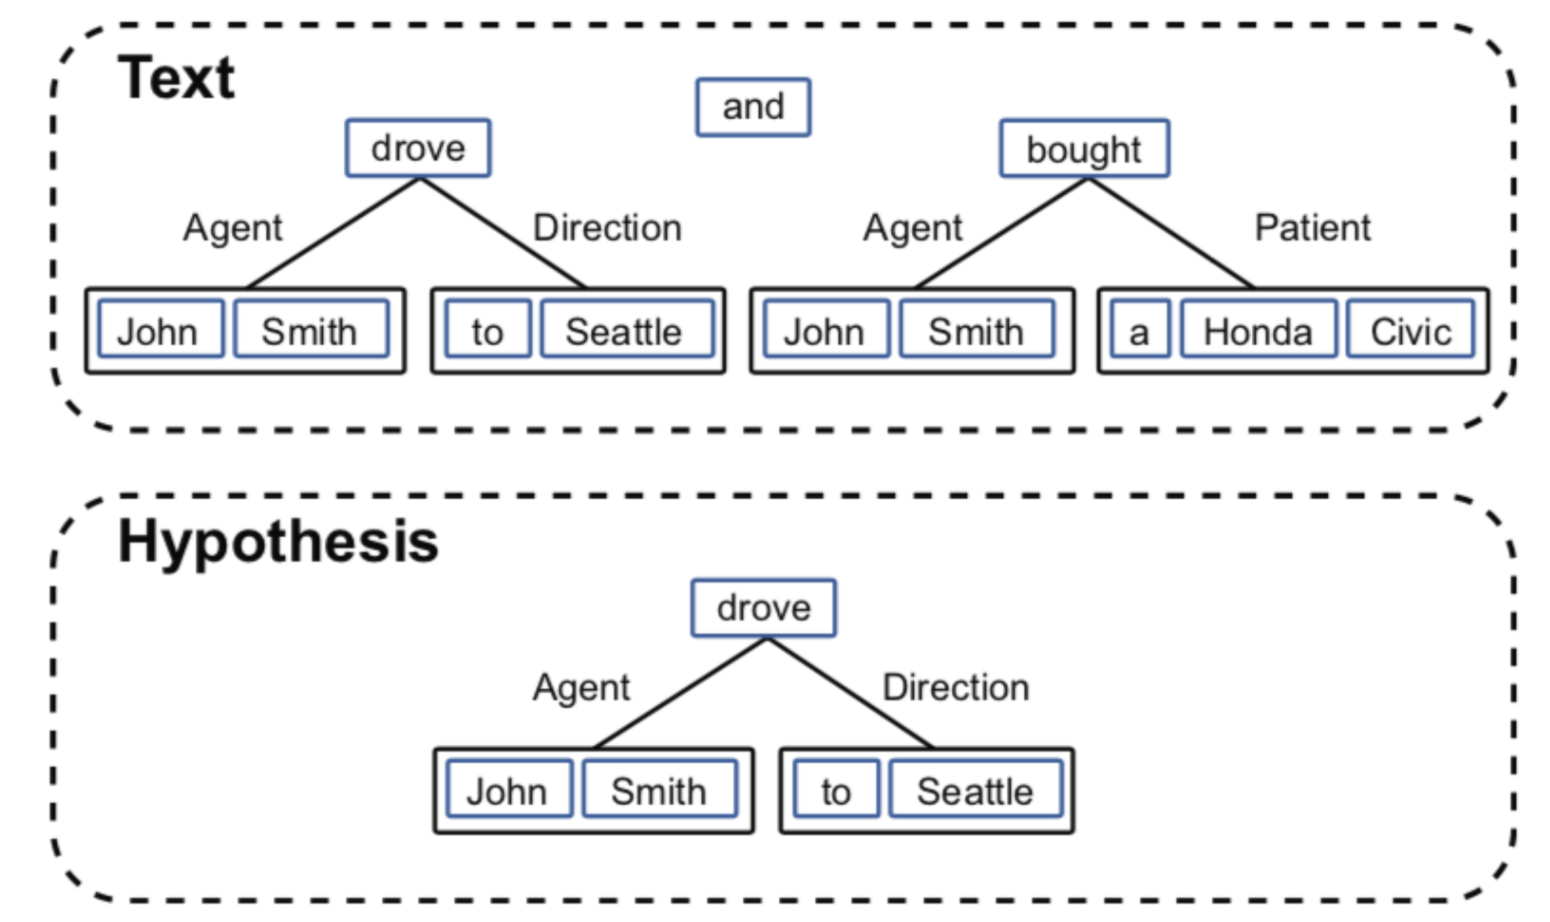
\includegraphics[width=0.4\textwidth]{figures/text_entailment_semantic_level.png}
		\end{figure}
	\end{itemize}
	\item \textbf{Knowledge Acquisition for RTE}
	\begin{itemize}
		\item To answer some text entailments, background/world knowledge is required (which words are synonyms, what is connected to a certain noun as i.e. a person/place...)
		\item Knowledge is mostly constrained to lexical-semantic between two words (synonym, hypnonymy, ...)
		\item But we can also model more complex relations like $X$ causes $Y$ $\implies$ $Y$ is a \textit{symptom} of $X$
		\item Such connections/knowledge can be retrieved from WordNet, Wikipedia, ...
		\item This leads to the \textbf{Extended Distributional Hypothesis}: if two paths occur in similar contexts, the meaning of the paths tend to be similar ($X$ \textit{solves} $Y$ compared to $X$ \textit{is a solution of }$Y$)
	\end{itemize}
\end{itemize}
\subsection{Recognizing Text Entailment Methods}
\begin{itemize}
	\item RTE depend on the representation which is used for $T$ and $H$
	\item Different approaches to model the classifier
	\item \textbf{Similarity-based approach}
	\begin{itemize}
		\item Pair with strong similarity score gets high entailment relation
		\item Similarity is measured by for example WordNet (how many edges to traverse to get to other word) and string similarity (length or even single letters)
	\end{itemize}
	\item \textbf{Alignment-based approaches}
	\begin{itemize}
		\item Use heuristics to align junk of words from $T$ to $H$
		\item For example, match phrase "\textit{purchase of $X$ to $Y$}" with "\textit{$Y$ acquired $X$}"
		\item However, we need a knowledge base to infer these relations
		\begin{figure}[ht]
			\centering
			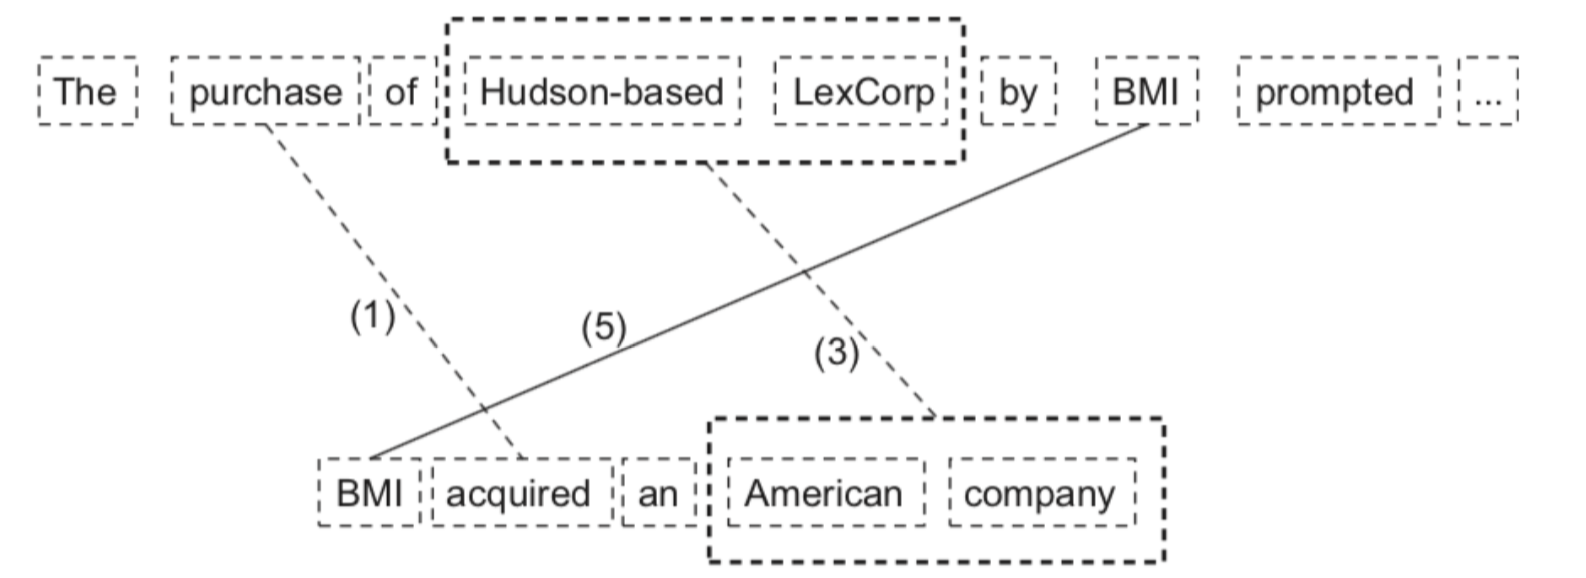
\includegraphics[width=0.4\textwidth]{figures/text_entailment_alginment_based_methods.png}
		\end{figure}
	\end{itemize}
	\item \textbf{Formal Logic approaches}
	\begin{itemize}
		\item Finding proof by theorem prover that $H$ can be proofed by $T$ 
		\item Convert statements in $T$ and $H$ into formal logic
		\item Problem: mostly the lack of background knowledge is the bottleneck, as the simplest mistakes/missing statements can stop this approach to get the correct result
	\end{itemize}
	\item \textbf{Edit distance-based approaches}
	\begin{itemize}
		\item Sequence of transformations that need to be applied on $T$ to get to $H$
		\item If the number of transformations is higher than specified threshold, classify relation as \texttt{false}
		\item Alternative for \textit{expensive} theorem prover
	\end{itemize}
	\item Evaluation done on dataset with 1,600 $T$-$H$ pairs with accuracy as metric. Lexical baseline is at about 58\%
\end{itemize}
\subsection{Current methods}
\begin{itemize}
	\item RTE datasets are mostly very small which limits the application of complex systems
	\item However, there are large Natural Language Inference datasets, where also neural networks can be trained on (different domains, for example image to text)
	\item We need datasets over multiple domains as otherwise the algorithms generalize poorly
	\item \textbf{Neural networks}
	\begin{itemize}
		\item Specifying features by hand for the input
		\item Using both hypothesis and text as input. Mostly, we classify then into classes \textit{entailment}, \textit{contradiction} and \textit{neutral} (not enough info to decide)
		\item Using various LSTM models with attention modules 
		\item Generative models create a hypothesis given the text and the class for which the hypothesis should be generated
		\item However, networks show to overfit on noise in the data (contradiction mostly contains negative words, entailments biased on animals and so on)
	\end{itemize}
\end{itemize}
\section{Computational Dialog Modeling}
\subsection{Modular dialog systems}
\begin{itemize}
	\item There are two main tasks in dialog modeling: either understand a conversation from outsider's view (summarizing), or the capability to take part in conversation $\Rightarrow$ make a dialog agent
	\item First approaches of modeling dialog agent were based on hand-specified patterns/transformation rules based on keywords to find an appropriate answer
	\item Recently, the focus shifted towards data-driven methods by either retrieving existing information or generating new sentences by i.e. Encoder-Decoder architectures
	\item Problems: hard to evaluate, such systems often show to just copy patterns in training dataset but don't generalize well.
	\item Different approach: in dialogs, there is a tendency to ascribe goal and \textbf{intentions}
	\item However, intentions are not easy to recognize. That's why such methods are often used for \textbf{task-oriented} dialog systems where the end-goal makes intentions tractable
	\item The modular dialog system architecture: 
	\begin{figure}[ht]
		\centering
		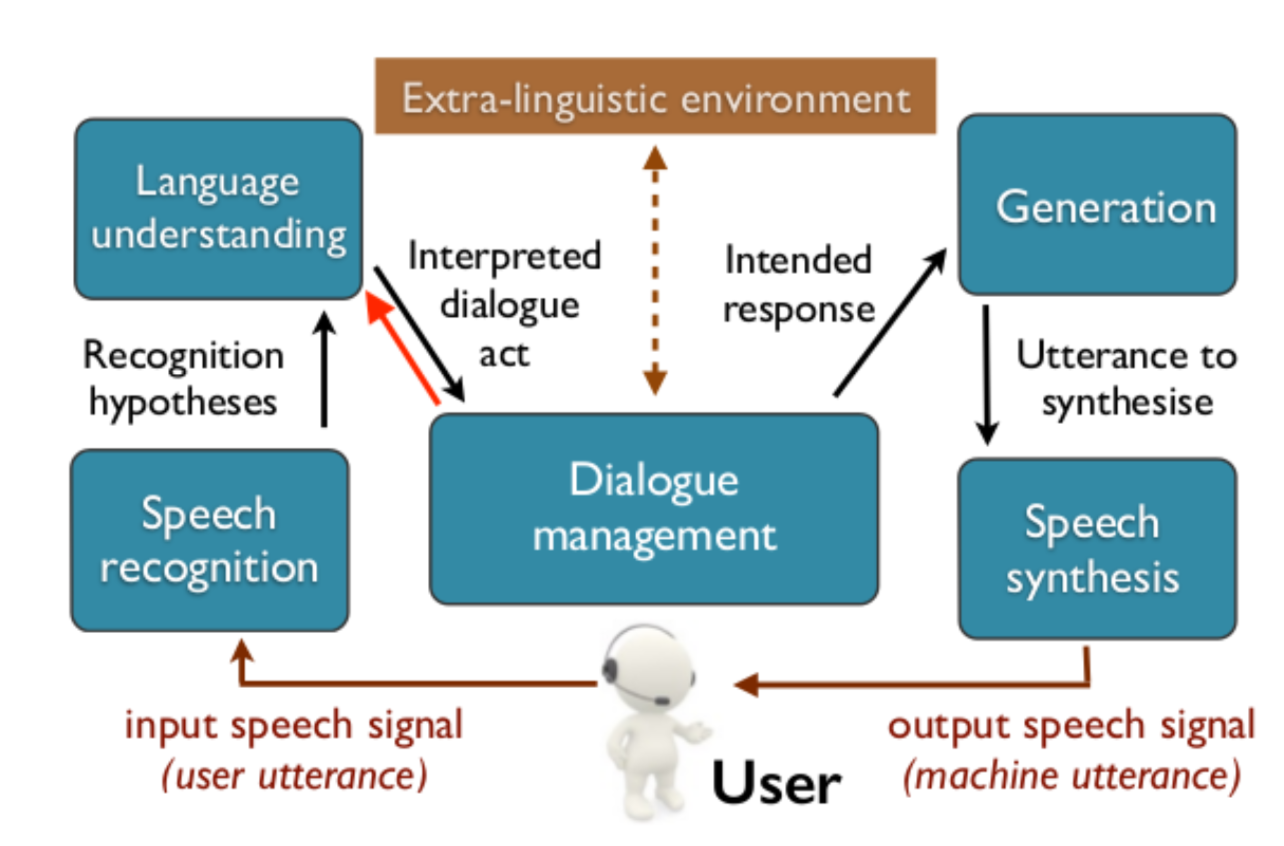
\includegraphics[width=0.4\textwidth]{figures/dialog_modeling_modules.png}
	\end{figure}
	\item \textit{Language understanding}: NLP1 course. Morphology, POS tagging, lexical semantics and syntactic parsing, compositional semantics, ...
	\item \textit{Dialog management}: consists of two modules:
	\begin{itemize}
		\item \textit{Dialog state tracker}: handle linguistic context (what has been said) and how relevant it is to the task. We can convert messages into slots with parameters (like \texttt{request(name)}) to simplify the task. 
		\item \textit{Dialog policy}: select what action to take next/model the next answer. Estimate probabilities for possible actions, and choose best ones. Training mostly done in a reinforcement learning way with simulator
	\end{itemize}
	\item \textit{Extra-linguistic environment}: taking information into account which is not coming from this dialog itself (images, databases, ...)
\end{itemize}
\subsection{Visually grounded, task-oriented dialog}
\begin{itemize}
	\item \textbf{Visual dialog}: given an image and a history of human-dialog, answer a follow-up question 
	\item We can evaluate this task with the same metrics as for summarization and translation (BLEU, ROGUE)
	\item However, in this task the agent is thrown at random into a conversation without being able to interact
	\item \textit{Image guessing game}: one agents ($Q$) sees the original image, and the other agent ($A$) sees the image with the object highlighted that $Q$ needs to guess
	\item Current implementation is based on LSTMs with CNN encoders. Still, the models perform poorly compared to humans
\end{itemize}
\section{Language generation and summarization}
\begin{itemize}
	\item Most tasks/methods until now have concentrated on language analysis. Next coming: tasks where we have to generate text
	\item Generation mostly has the starting point at semantic representation like distributional semantics or hidden representation for neural networks
	\item We can also concentrate on \textit{regeneration} where we convert input to another representation. Examples include summarization, translation, ...
	\item For generation, there are various subtasks (e.g. content selection, discourse structuring, ...)
	\item Approaches for generation include:
	\begin{itemize}
		\item \textit{Templates}: fixed text that has slots that can be filled
		\item \textit{Statistical}: using machine learning
		\item \textit{Deep Learning}: using deep embeddings, especially for regeneration task
	\end{itemize}
\end{itemize}
\subsection{Text Summarization}
\begin{itemize}
	\item Task: generate short version of input text with important points
	\item We distinguish between \textbf{single-document summarization} (given a single document, produce summary with important points) and \textbf{multi-document summarization} (given a set of documents, produce brief summary of combination)
	\item Also, we differentiate between \textbf{generic summarization} (identifying important parts by itself and present these) and \textbf{query-focused summarization} (regarding a query/question from the user, find relevant parts in the document/s)
	\item There are mostly main approaches:
	\begin{itemize}
		\item \textbf{Extractive summarization}: extract important info from document by copying sentences and combine them into a summary
		\item \textbf{Abstractive summarization}: interpret content of document and generate completely new sentences (much harder task!)
	\end{itemize}
	\item Most approaches deal with extractive summarization as it is much easier to realize and achieves better results till now
\end{itemize}
\subsubsection{Extractive summarization}
\begin{itemize}
	\item For extractive summarization, there are three main steps:
	\begin{enumerate}
		\item \textbf{Content selection}: identify important parts/sentences from the document 
		\item \textbf{Information ordering}: order the sentence within the summary
		\item \textbf{Sentence realization}: optimizing the text by e.g. sentence simplification
	\end{enumerate}
	\item Approaches for \textit{content selection}
	\begin{itemize}
		\item \textit{Unsupervised}: 
		\begin{itemize}
			\item Take those words that are significantly more often used than in other documents in average $\Rightarrow$ these are the ``informative'' words and mostly biased towards names/cities (pronoun resolution important to find these references as well)
			\item Measured by metrics like \texttt{tf-idf}
		\end{itemize}
		\item \textit{Supervised}:
		\begin{itemize}
			\item Large training corpus with human summary needed
			\item Sentences of summary are aligned with those in the original document, and features are extracted (position in document, sentence length, informative words, ...)
			\item Based on these features, we train a binary classifier whether a sentence should be included in the summary or not
			\item Problem: expensive to generate all this data, and the supervised approaches did not significantly outperform the unsupervised ones
		\end{itemize}
	\end{itemize}
	\item Approaches for \textit{information ordering}:
	\begin{itemize}
		\item For a single document, the sentences are mostly structured in the order they occur in the original document
	\end{itemize}
\end{itemize}
\subsubsection{Query-focused multi-document summarization}
\begin{itemize}
	\item For query-focused multi-document summarization, we need to extend the extractive summarization by two pre-processing steps:
	\begin{enumerate}
		\item Find a set of relevant documents
		\item (Optionally) simplify sentences in the documents (to make the task of content selection easier)
		\item \textit{Content selection}: identify informative sentences in the documents (much harder than for the single-document task)
		\item \textit{Information ordering}: order the sentences in the summary
		\item \textit{Sentence realization}: modify sentences to get consistent summary
	\end{enumerate}
	\item Approaches for \textit{sentence simplification}
	\begin{itemize}
		\item Parse sentences and apply hand-rules what parts of a sentence we might drop (initial adverbials as ``for example'', irrelevant attribute clauses, ...)
		\item Also possible to train a classifier to identify satellites (non-informative parts on a nucleon phrase)
	\end{itemize}
	\item Approaches for \textit{content selection} for multiple documents
	\begin{itemize}
		\item We can either combine all documents into one, or retrieve information from all documents separately and weight these documents
		\item Estimate informativeness similarly to single-document
		\item Then, start by adding the most informative sentences in summary (one by one) until the maximum length of the summary is reached
		\item When adding new sentences, we need to make sure that not the same/very similar sentences from different documents are added $\Rightarrow$ \textbf{Maximum marginal relevance}
		\begin{itemize}
			\item Iterative method to determine best sentence to add to summary. Relies on two counter-part measures:
			\item \textit{Relevance to query}: high cosine similarity between a sentence and the query indicates a high relevance for the summary
			\item \textit{Novelty regarding the summary so far}: low cosine similarity between sentences and summary
			\item Estimated score is calculated as follows (for query $Q$, summary $S$, documents $D$):
			$$\hat{s} = \arg\max_{s_i \in D} \left[\lambda \text{sim}\left(s_i, Q\right) - \left(1 - \lambda\right)\max_{s_j \in S}\text{sim}\left(s_i, s_j\right)\right]$$
		\end{itemize}
	\end{itemize}
	\item Approaches for \textit{sentence ordering}
	\begin{itemize}
		\item \textit{Chronologically}: for example by date of document
		\item \textit{Coherence}: sentences that are similar/discuss same entity should be grouped together in the summary
		\item \textit{Topical ordering}: learns set of topics present in documents (by e.g. topic modeling), and then order the sentences by topic
	\end{itemize}
\end{itemize}
\subsubsection{Summarization using neural networks}
\begin{itemize}
	\item We can apply neural networks for the task of summarization
	\item For extractive summarization, we train a RNN on word level creating a representation of words, and a RNN on sentence/document level that combines sentence embeddings
	\item Apply classifier on output of all document-level RNN to decide whether to include sentence in summary or not (problem: still captures coarse-grained features)
	\begin{figure}[ht]
		\centering
		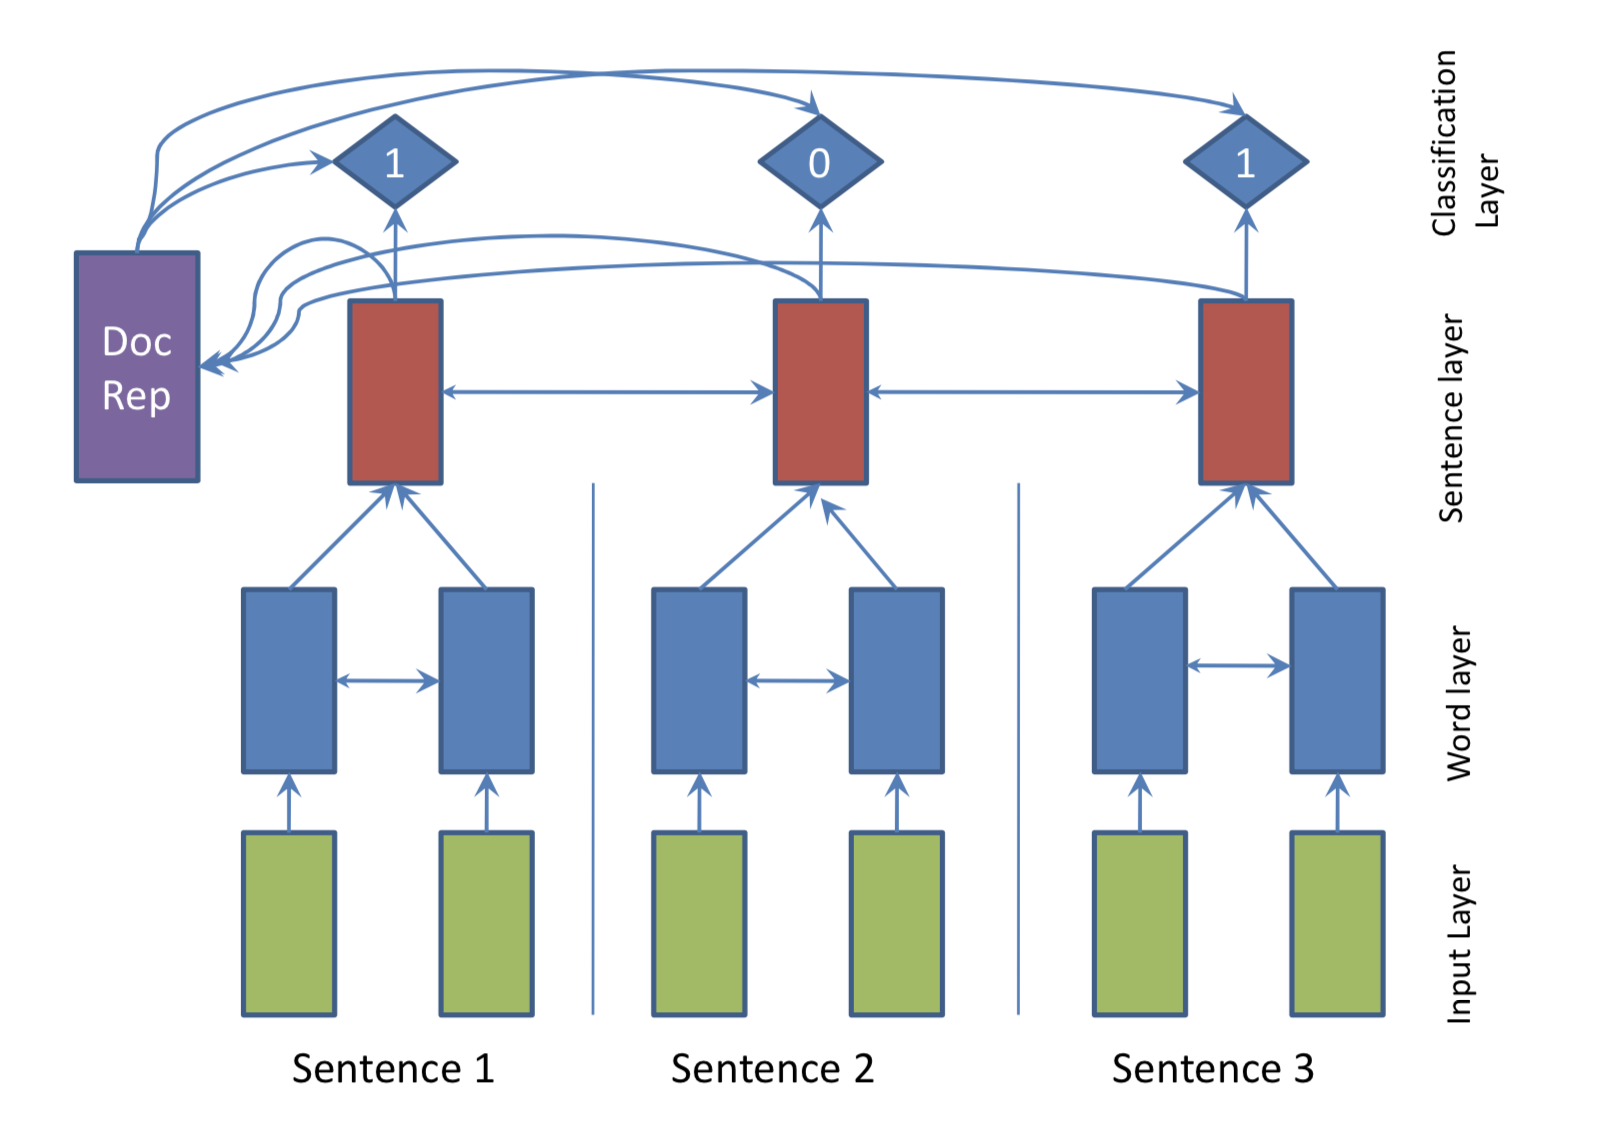
\includegraphics[width=0.3\textwidth]{figures/summarization_rnn.png}
		\caption{Summarization by RNNs}
		\label{fig:summarization_rnn}
	\end{figure}
	\item Abstractive summarization can be realized by large newspaper datasets where for a small article, a headline must be predicted
	\item We use an Encoder-Decoder architecture (seq2seq models) where the encoder generates fixed-size embedding, and the decoder generates word-by-word output given this representation (decoder is autoregressive as it takes own output back as input for next time step)
\end{itemize}
\subsubsection{Evaluating summarization models}
\begin{itemize}
	\item Human judgments of quality is too expensive
	\item Better, automatic method: \textbf{ROUGE} (recall oriented understudy for gisting evaluation)
	\item We compare a few human-generated summaries $R_1, ..., R_N$ with the system generated summary $S$ by computing the percentage of $n$-grams from the reference summaries $R_1,...,R_N$ that occur in $S$. Example: ROUGE-2 (using bigram):
	$$\frac{\sum_{R_i}\sum_{bigram_j\in R_i} \text{count}_{\text{match}}(j,S)}{\sum_{R_i}\sum_{bigram_j\in R_i} \text{count}(j, R_i)}$$
	\item Note that summary length is not considered here 
	\item Example for calculating ROUGE metric:
	\begin{figure}[ht]
		\centering
		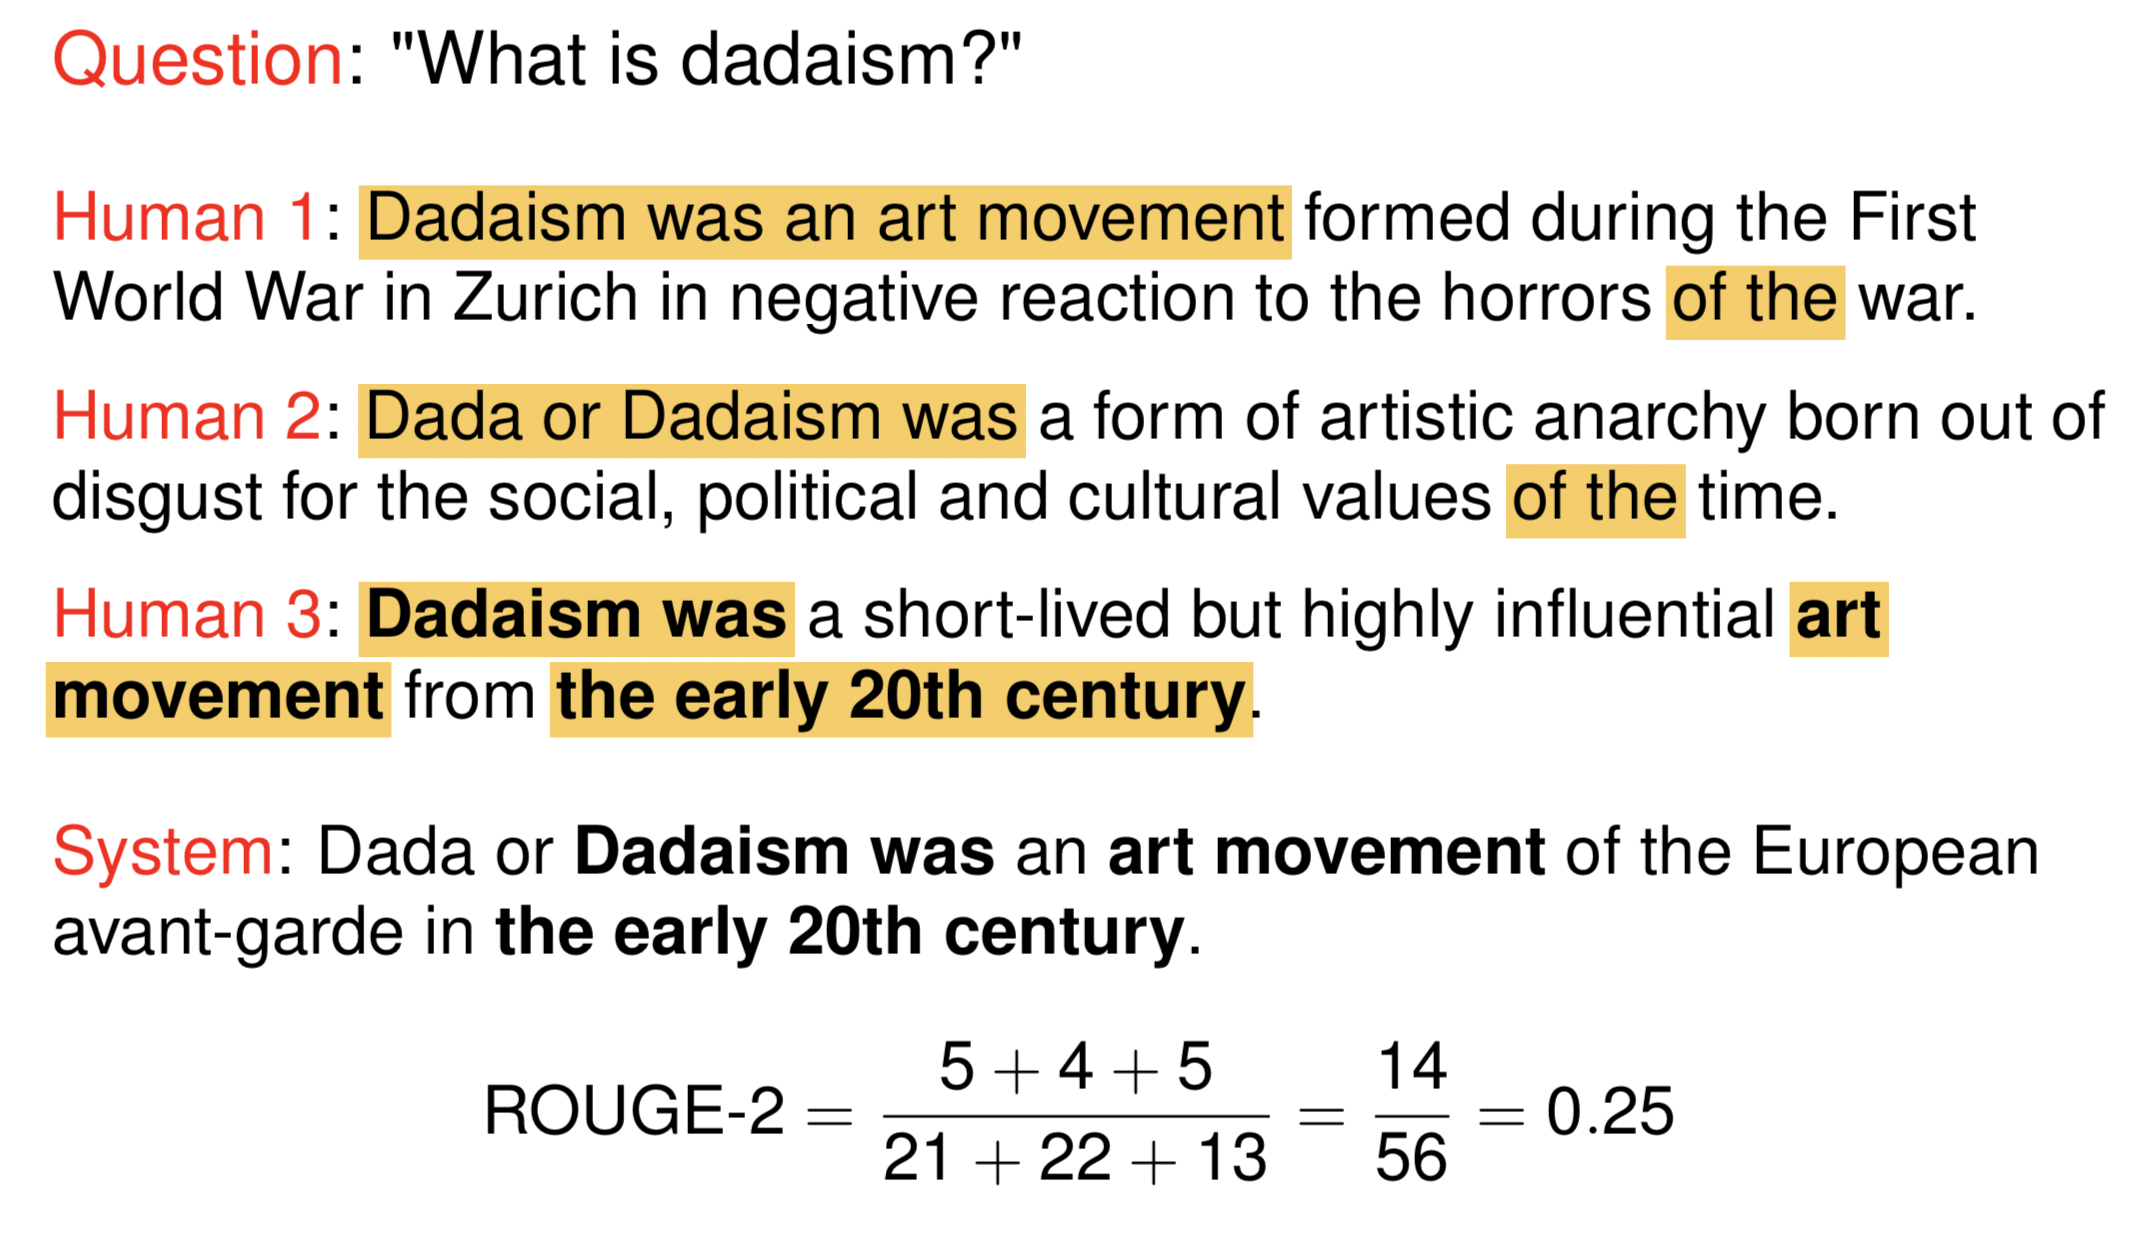
\includegraphics[width=0.5\textwidth]{figures/summarization_rogue_example.png}
		\label{fig:summarization_rogue_example}
	\end{figure}
	% summarization_rogue_example.png
\end{itemize}
\section{Machine Translation}
\subsection{Statistical Machine Translation}
\begin{itemize}
	\item Given a sentence $f$ in foreign language, find most probable translation $\hat{e}$:
	$$\hat{e} = \arg\max_{e} P(e|f) = \arg\max_{e} \underbrace{P(f|e)}_{\text{channel}} \underbrace{P(e)}_{\text{source}}$$
	\item The source is the \textbf{language model} which makes sure that the grammatical structure in the text is correct
	\begin{itemize}
		\item It is also helpful for disambiguate the word decision in the translating language
		\item This is very important if a word in the foreign language is ambiguous
	\end{itemize}
	\item The (noisy) channel is the \textbf{translation model} which is responsible to translate the text (makes sure that $f$ are translations of $e$)
	\item IBM-3 model:
	\begin{itemize}
		\item For every word:
		\begin{itemize}
			\item Choose a fertility $\phi_i$ (number of words in goal language should be translated into in foreign language. E.g. ``did'' has fertility of 0, ``slap'' 3 in French)
			\item Generate $\phi_i$ foreign words
			\item Generate spurious/default words that might be needed
		\end{itemize}
		\item Permute translated words based on the position a word was before, and language it was in before
	\end{itemize}
\end{itemize}
\subsubsection{Learning parameters of models}
\begin{itemize}
	\item For learning the parameters of the language and translation model, we would need the word alignments in the translation which however require the parameters
	\item Thus, we apply the Expectation-Maximization algorithm
	\item Assume we have alignments, but for every sentences multiple ones. For example, we can have the following possible alignments for a two-word sentence:
	\begin{figure}[ht]
		\centering
		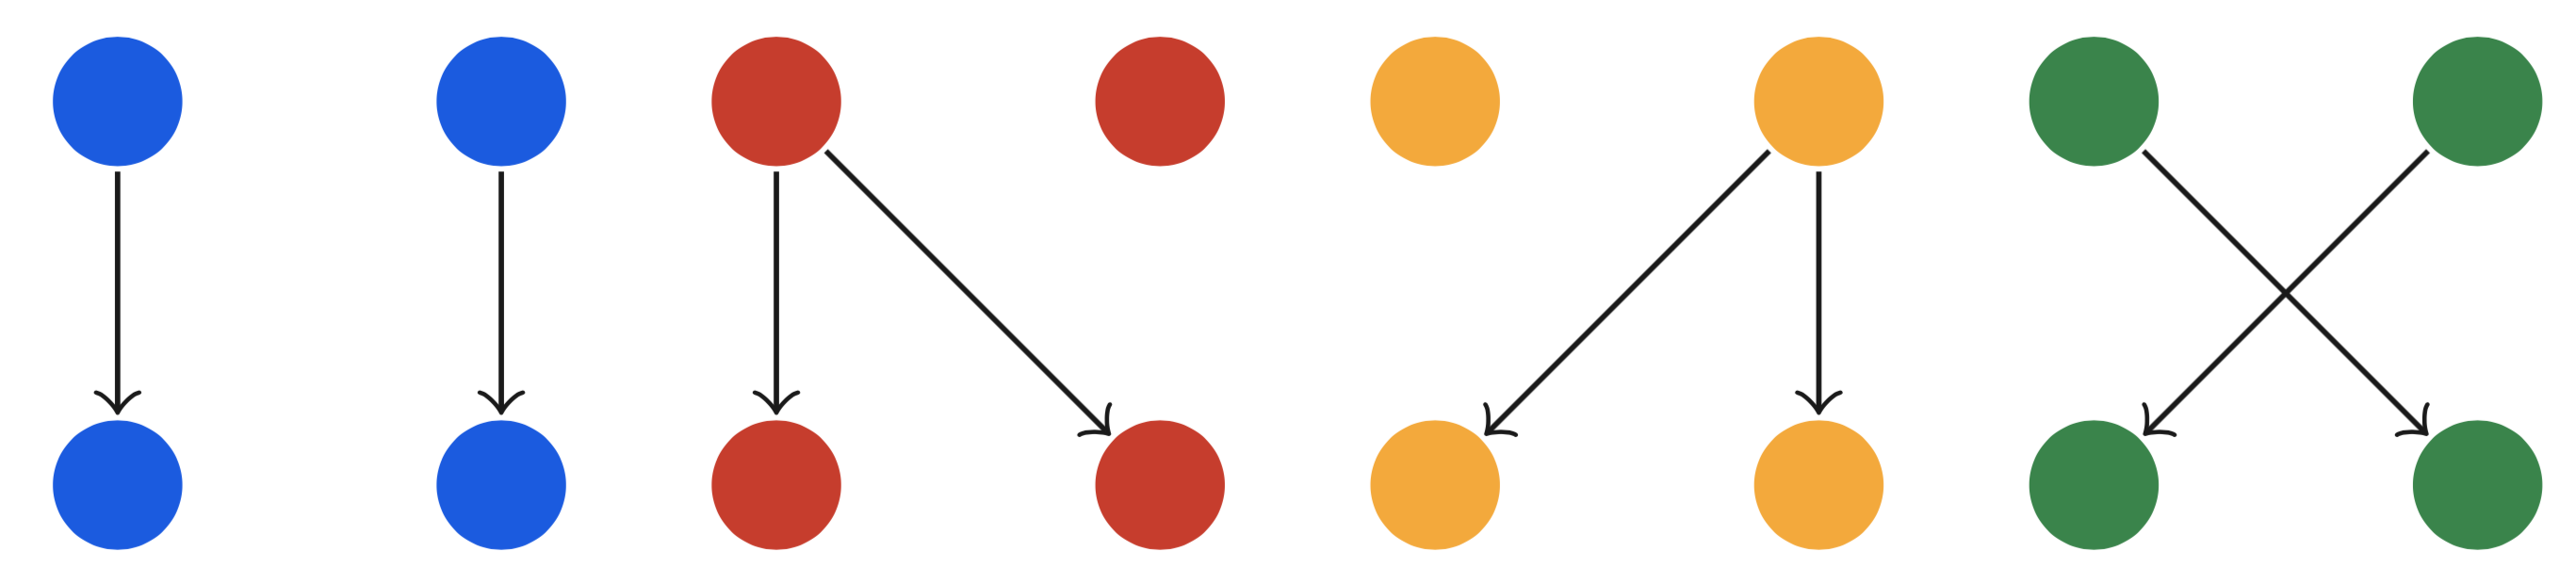
\includegraphics[width=0.5\textwidth]{figures/translation_EM_alignment.png}
	\end{figure}
	\item Every alignment is assigned to a probability/fractional count it occurs. Initially, we set the probability of every alignment/word to a uniform distribution
	\item We try to maximize the probability that a foreign word/phrase $f_j$ in our corpus is  a translation of $e_{a_j}$ where $a_j$ is the alignment of the foreign to translated language. When using Bayes rule (and looking at only 1to1 alignments), we maximize:
	$$P(a,f|e) = \prod\limits_{j=1}^{M}t(f_j|e_{a_j})$$
	where $t$ are the fractional counts
	\item EM algorithm:
	\begin{enumerate}[label=Step \theenumi:]
		\item Compute $P(a,f|e)$ for every possible alignment and sentence
		\item Normalize the alignments for the same foreign sentence. $P(a,f|e)\to P(a|f,e)$
		\item Collect the fractional counts $tc(x|b)$ by summing up the probabilities of all $P(a|f,e)$ where $b$ is aligned to $x$. 
		\item Normalize fractional counts by $b$ $\Rightarrow$ revised parameters for next iteration
	\end{enumerate}
	\item Example: Given $t(x|b) = 1/4$, $t(x|c)= 3/4$, $t(y|b)= 1/2$, $t(y|c)= 1/2$.
	\begin{figure}[ht]
		\centering
		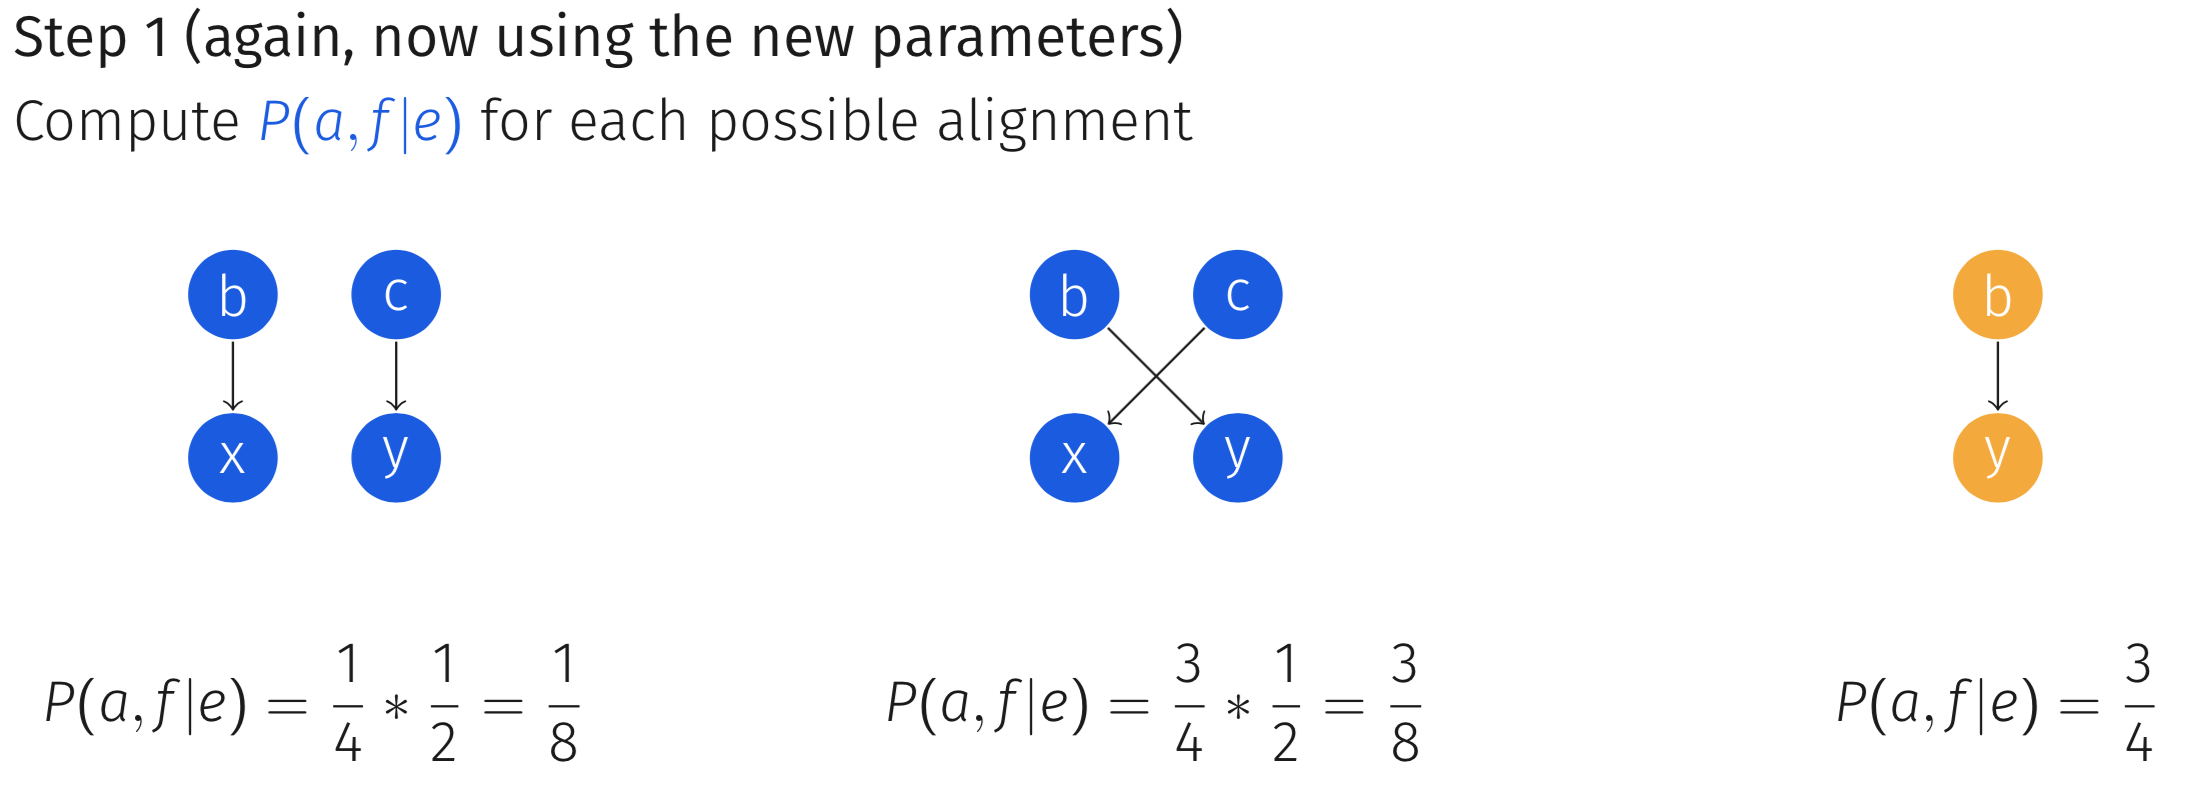
\includegraphics[width=0.5\textwidth]{figures/translation_EM_step_1.png}
	\end{figure}
	\begin{figure}[ht]
		\centering
		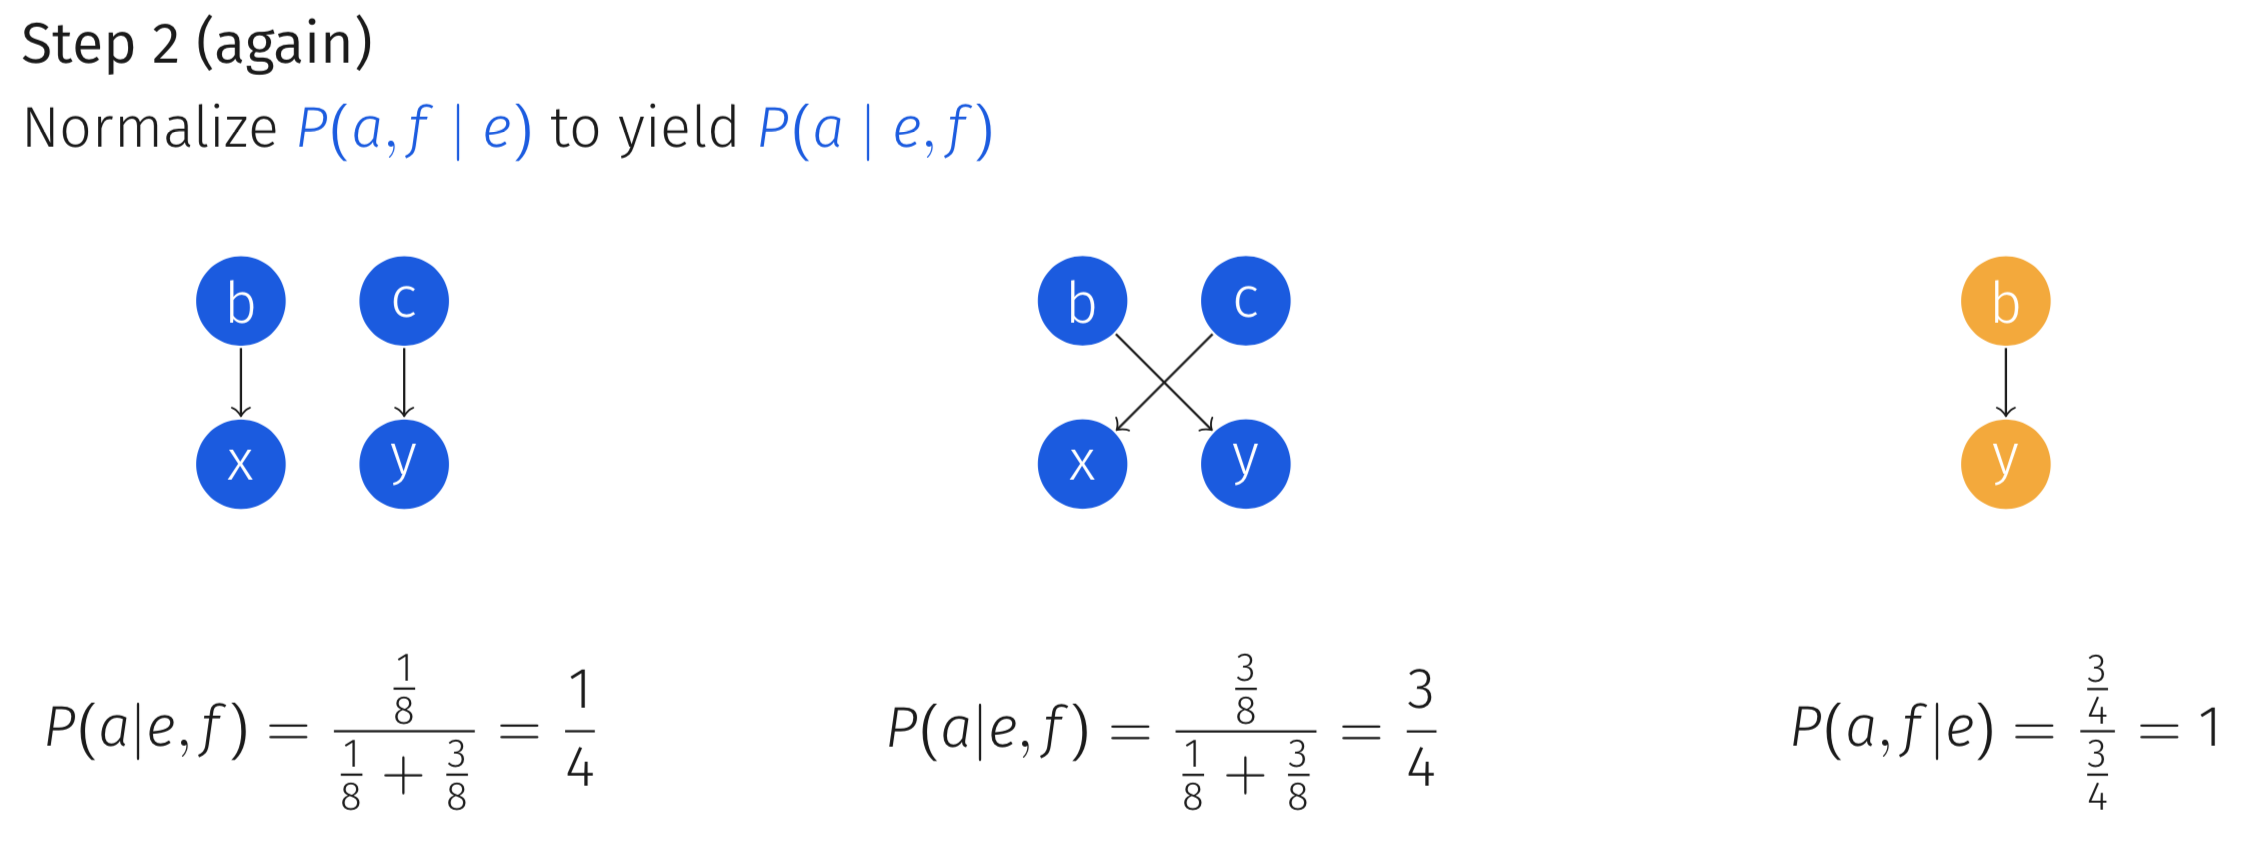
\includegraphics[width=0.5\textwidth]{figures/translation_EM_step_2.png}
	\end{figure}
	\begin{figure}[ht]
		\centering
		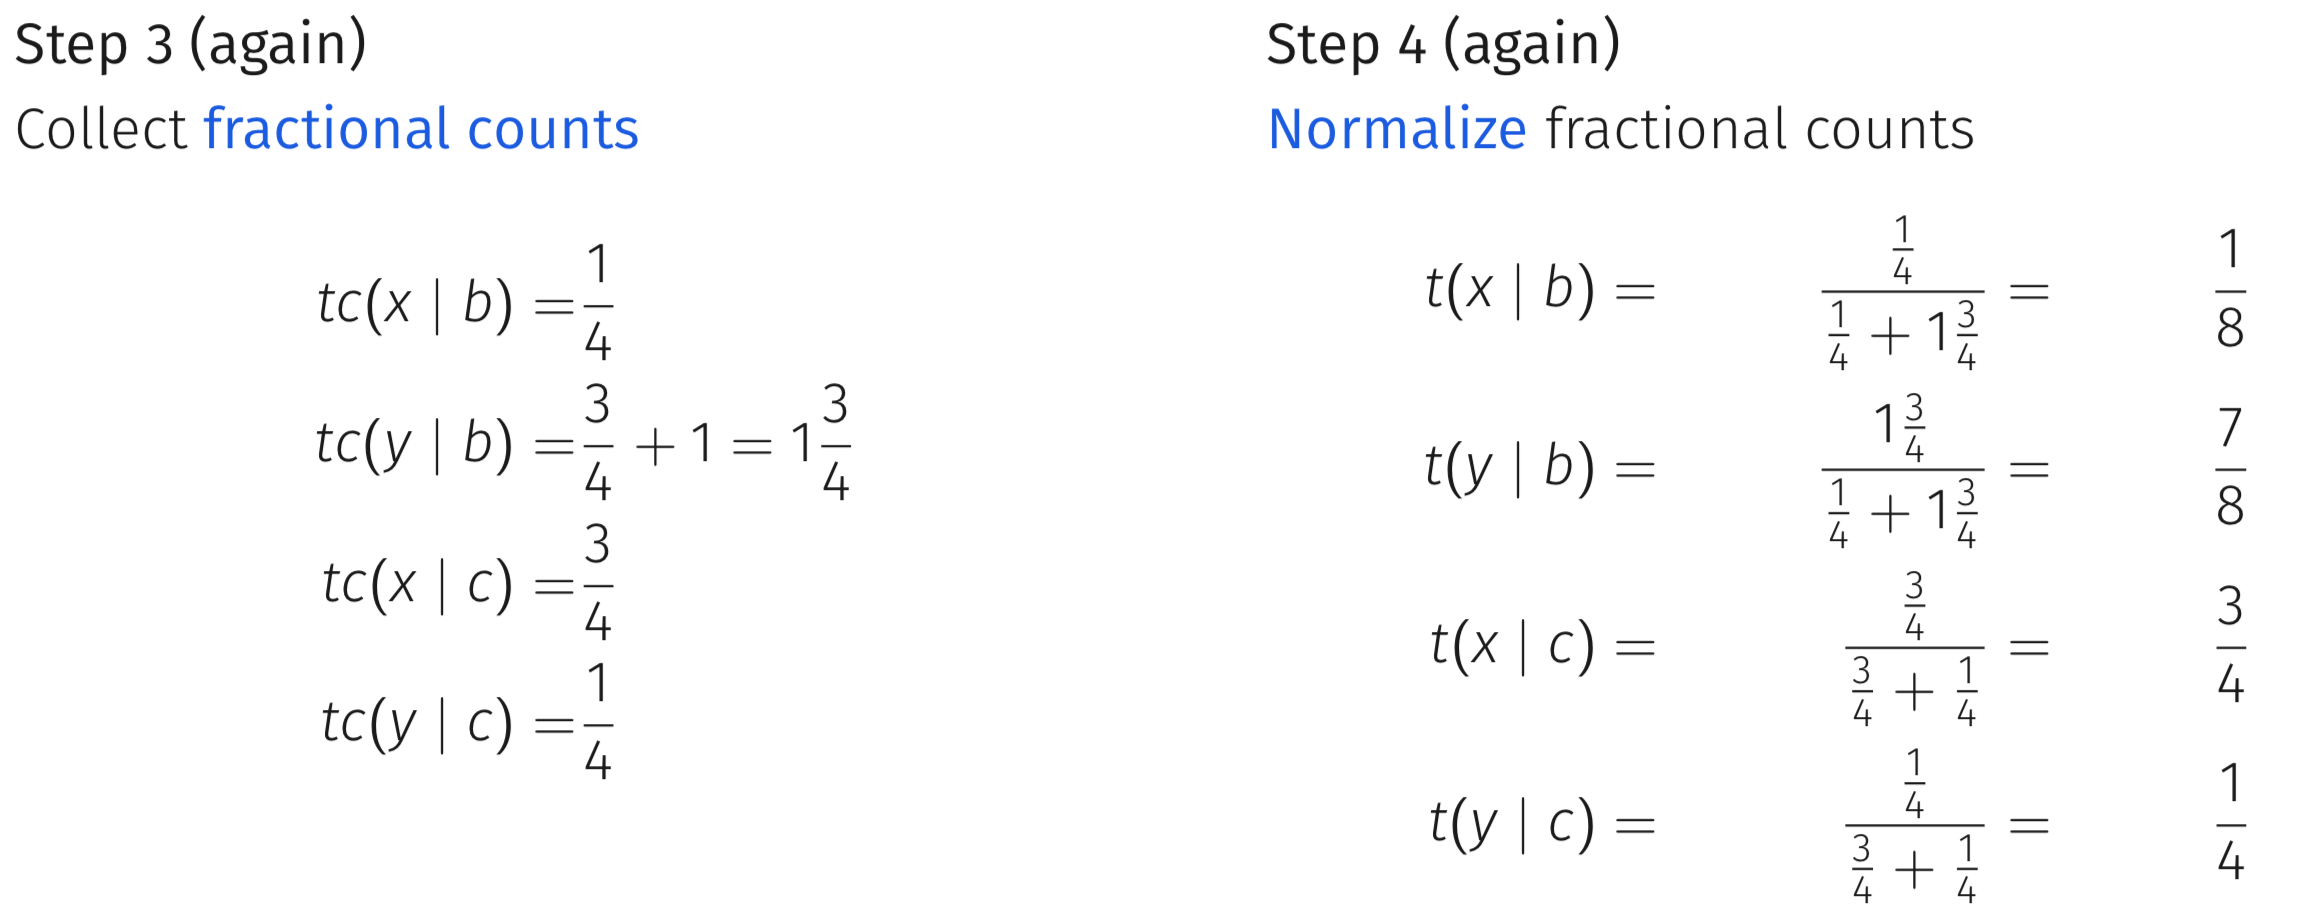
\includegraphics[width=0.5\textwidth]{figures/translation_EM_step_3_4.png}
	\end{figure}
	\item Note on EM: Optimization function is non-convex so that we might find a local minimum
\end{itemize}
\subsection{Phrase-based Statistical Machine Translation}
\begin{itemize}
	\item Previously, translation was based on single words as atomic unit. However, we can also use phrases (few consecutive words) as unit 
	\item The advantage is that context can be taken into account for translation, and no more fertility, insertion and deletion of words are necessary to translate
	\item We now have a phrase table where we have probabilities to translate a certain phrase into another
	\item The translation model uses phrases instead of words, but also needs to consider to reorder the phrases:
	$$P(f|e) = \prod\limits_{i=1} \phi(\overline{f}_i | \overline{e}_i) \underbrace{d(\text{start}_i - \text{end}_i -1)}_{\text{distance-based reordering}}$$
	Note that $\text{start}$ and $\text{end}$ are the positions in the foreign language, but $i$ is the index of the translated language!
	\item Extract all phrases that are consistent with a word alignment $A$. A phrase is consistent if all words of $\overline{f}'$ are only aligned to words in $\overline{e}'$ and not any other words outside this phrase (and the other way round).
	\item The \textit{phrase translation probability} $\phi$ is estimated by the relative frequency:
	$$\phi(\overline{f}, \overline{e}) = \frac{\text{count}(\overline{f}, \overline{e})}{\sum_i \text{count}(\overline{f}_i, \overline{e})}$$
\end{itemize}
% \section{Foundations of Bayesian NLP}
% \textbf{Foundations of Bayesian NLP is not in the exam.}
\appendix
% \newpage
% \input{nlp_appendix.tex}
\end{document}